% !TEX encoding = UTF-8 Unicode
% !TEX root = thesis-ex.tex
This chapter shall discuss some important experimental jet measurements that motivate the study of the main analysis in this thesis. These include the study of the jet yields, dijet asymmetry, and jet fragmentation. It shall then go on to discuss a few models that have been used to explain the data, looking in particular at the following: Effective Quenching (EQ), Soft Collinear Effective Theory (SCET), Hybrid Model, and Jet Fluid Model.


\section{Dijet Balance: $\mathrm{x}_{J}$}
\label{sec:xj}
This section will discuss the dijet balance for $R = 0.4$ jets as measured by ATLAS detector for \pbpb\ collisions at \sqrtsnn = 2.76 TeV \cite{Aaboud:2017eww}. The dijet imbalance can be expressed in terms of $x_J$ defined as

\begin{align}
x_J =  \frac{\pt_2}{\pt_1}
\end{align}

where $\pt_2$ and $\pt_1$ are the transverse momenta of the two highest-\pt\ jets in the event respectively. The minimum $\pt_2$ considered is 25 GeV and the pair of jets are separated by $|\Delta\phi| > 7\pi/8$. The dijet yields normalized by the number of jets and determined as $1/N_\mathrm{jets} dN/dx_J$ are presented as a function of $x_J$ for different centrality intervals, as well as different ranges for $\pt_1$. The measured distributions are further unfolded to remove detector resolution effects and allow comparison to theoretical models.

Figure~\ref{fig:xJ} shows the $x_J$ distribution for dijet pairs in \pp\ and \pbpb\ collisions in two different centrality bins and two $\pt_1$ ranges. It can be seen that the dijet yields in \pp\ are peaked at unity and become narrower for larger $\pt_1$ ranges. This reflects the fact that the effects of jet quenching are minimal and the higher-\pt\ jets are better balanced. The dijet yields in peripheral \pbpb\ collisions are similar to the distributions from the \pp\ data, showing that the effects of quenching are smaller. On the other hand, dijet yields in central \pbpb\ collisions are significantly broadened, reflecting the maximal  of jet quenching. This is consistent with the picture of the individual jets in the dijet pair traversing different lengths in the QGP and hence losing different amounts of energy. In fact, the distribution for \pbpb\ data is peaked at $x_J = 0.5$, implying a loss of 50\% of the jet \pt.

\begin{figure}[htbp]
\begin{center}
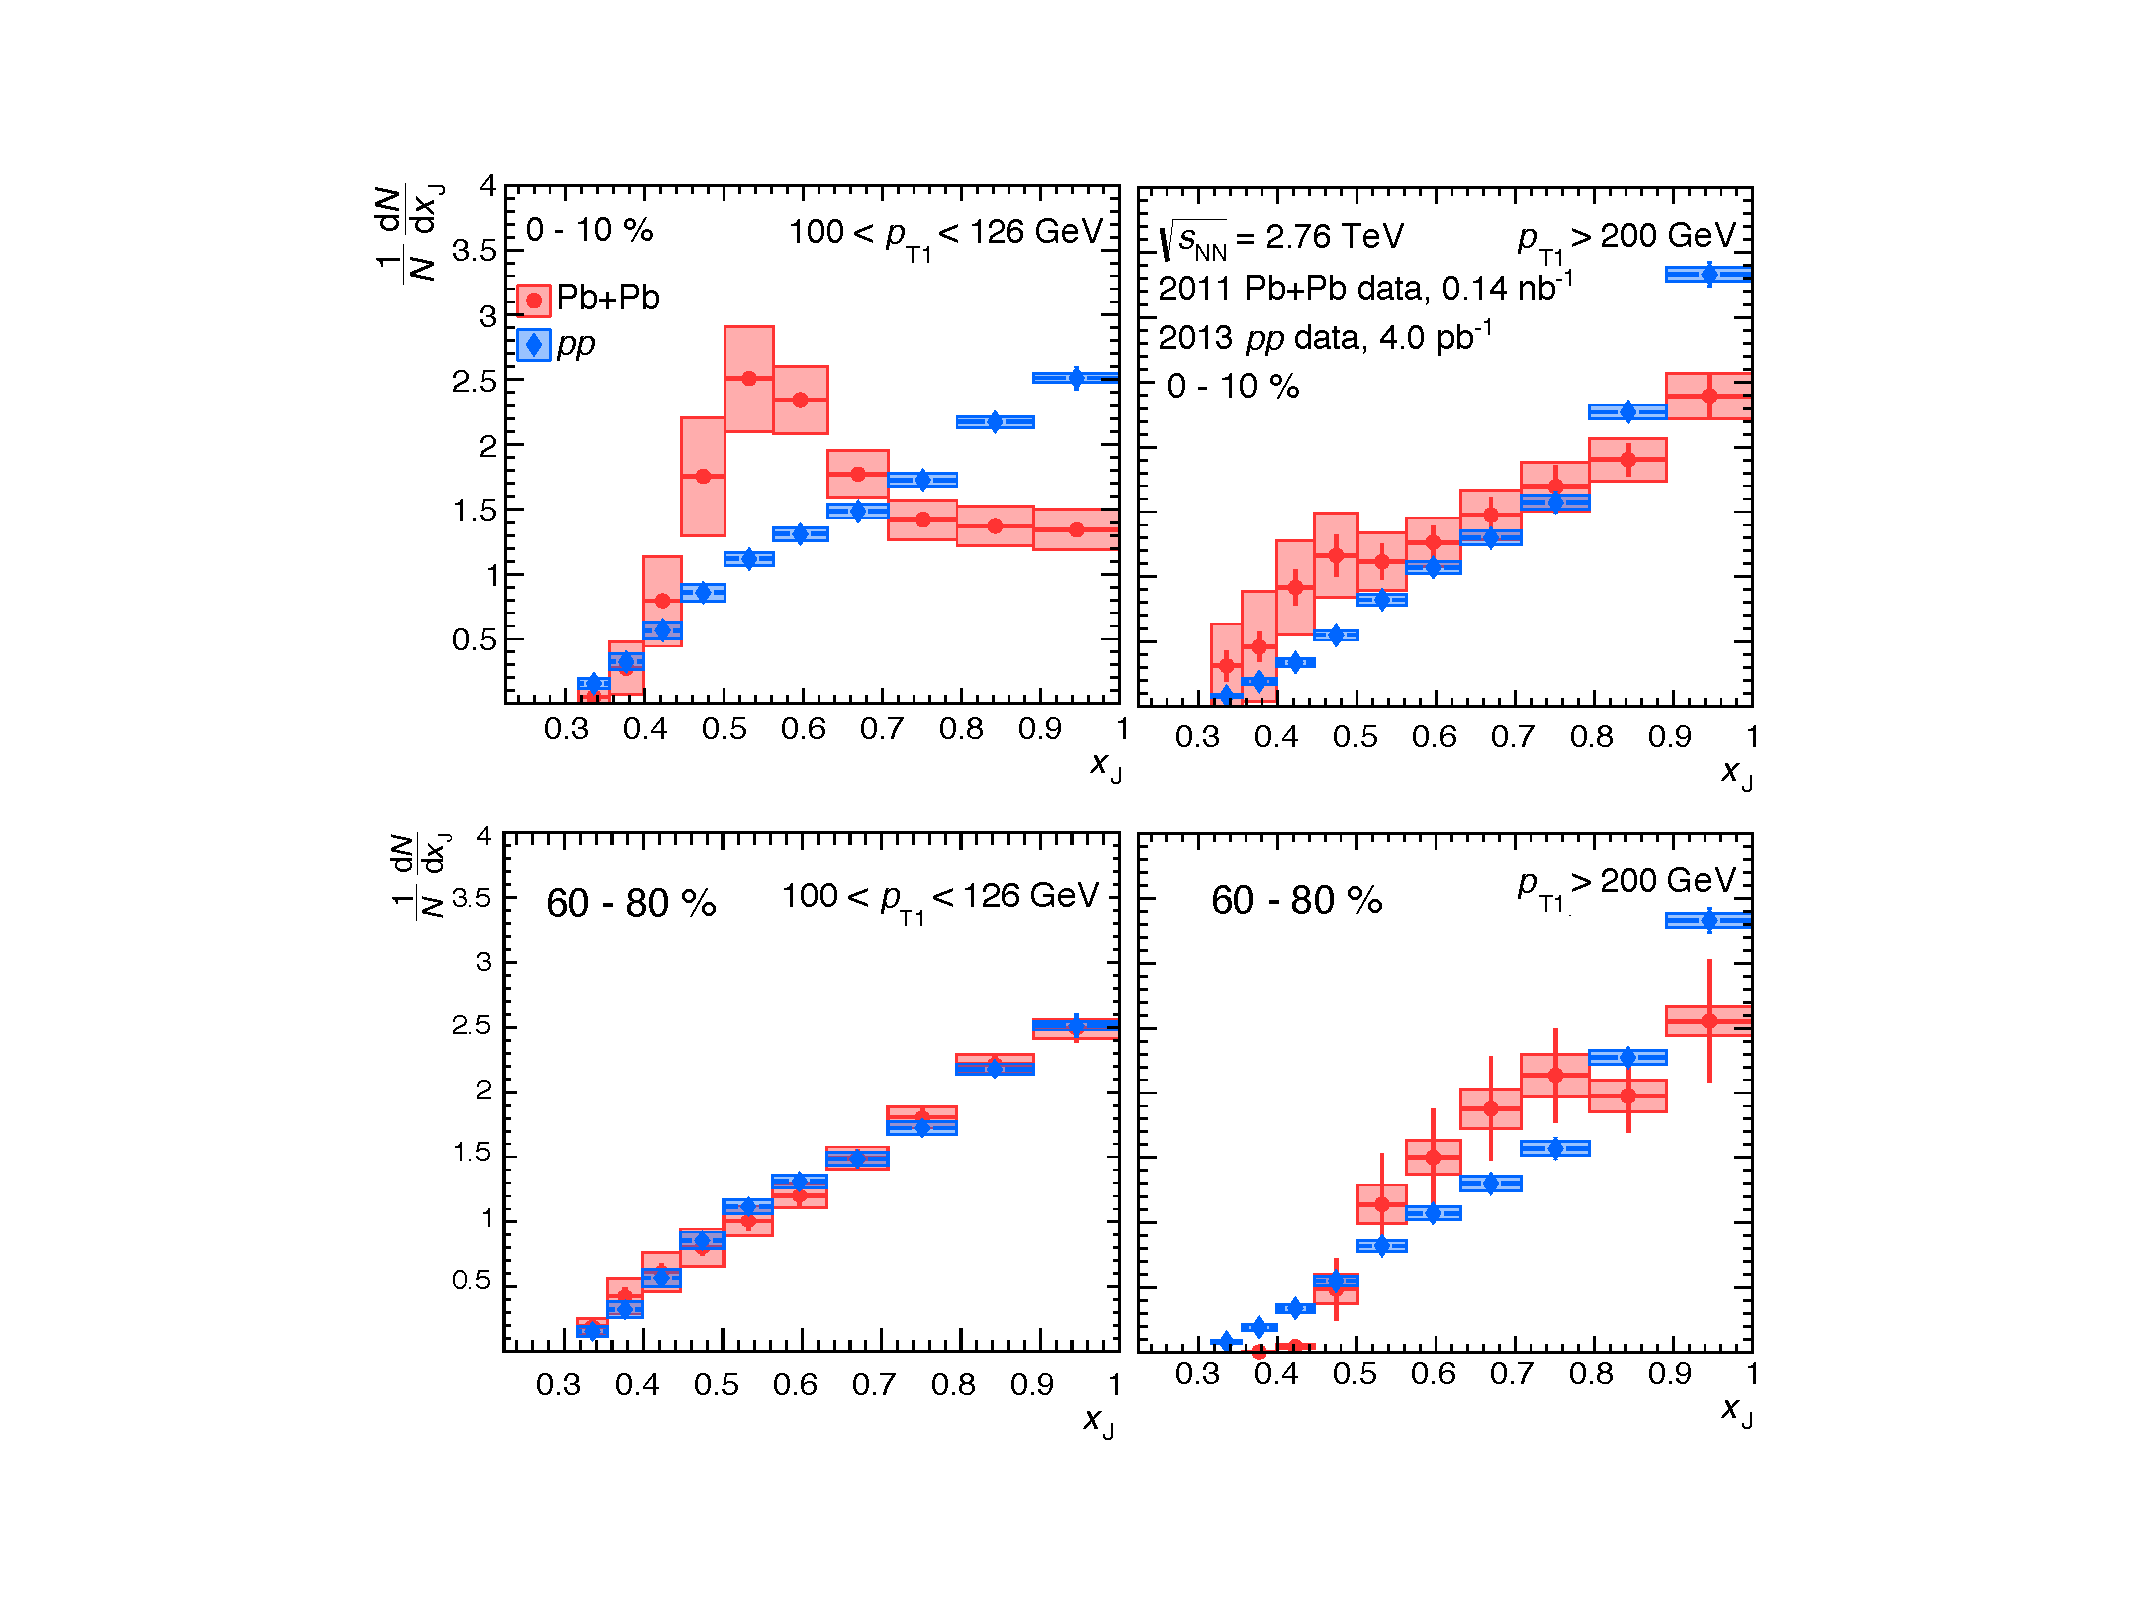
\includegraphics[width=0.55\textwidth]{figures/jetMeasurements/xJ}
\caption{The $1/N_\mathrm{jets} dN/dx_J$ distributions for $R=0.4$ jets as a function of $x_J$ for \pp\ (blue) and \pbpb\ (red) collisions. The different panels are for (top) central and (bottom) peripheral collisions in (left) $100 < \pt_1 < 126$ GeV and (right) $\pt_1 > 200 $ GeV. The \pp\ data is the same in all panels. The statistical uncertainties are indicated by the bars while the boxes indicate the systematic uncertainties. Figures taken from \cite{Aaboud:2017eww}}
\label{fig:xJ}
\end{center}
\end{figure}

Further measurements of $R = 0.3$ jets are shown in Figure~\ref{fig:xJ_R03}. These distributions are significantly flatter than the ones for $R=0.4$ jets, an observation that is consistent with the expectation that the transverse momenta correlation between the dijet pair is weaker for jets with smaller radii due to radiation that is outside the nominal jet cone.

\begin{figure}[htbp]
\begin{center}
\includegraphics[width=0.55\textwidth]{figures/jetMeasurements/xJ_R03}
\caption{The $1/N_\mathrm{jets} dN/dx_J$ distributions for $R=0.3$ jets as a function of $x_J$ in \pp\ and central \pbpb\ collisions. The different panels are for different, $\pt_1$ ranges (top left to bottom right) central and (bottom) peripheral collisions. The \pbpb\ data is in red circles while the \pp\ data is in blue diamonds and is the same in all panels. The statistical uncertainties are indicated by the bars while the boxes indicate the systematic uncertainties. Figures taken from \cite{Aaboud:2017eww}}
\label{fig:xJ_R03}
\end{center}
\end{figure}

%%%%%%%%%%%%%%%%%%%%%%%%%%%%%%%%%%%%%%
\section{Modification of jet yields: $\mathrm{R}_{AA}$}
\label{sec:jet_raa}

This section discusses the measurement of the inclusive jet \RAA\ as measured by the ATLAS detector for $R=0.4$ jets in $\sqrtsnn=5.02$ TeV \pbpb\ collisions \cite{2019108}.

While a measurement that compares the jets in a dijet system to each other as discussed in Section~\ref{sec:xj} can provide valuable information about how jets lose energy, it has the following limitation: If both jets lose equal amounts of energy, the dijet yield will still be peaked at unity and no new information will be obtained. Thus, it is useful to compare the jet yields directly between the \pp\ and \pbpb\ systems and construct the jet \RAA\ observable. This is defined as:

\begin{align}
\RAA  = \dfrac{\dfrac{1}{N_{\rm evt}} \left. \dfrac{d^2 N_{\rm jet}}{d\pt dy} \right|_{\rm cent}}{ \langle T_{\rm AA} \rangle \left. \dfrac{d^2\sigma_{\rm jet}}{d\pt dy} \right|_{\rm pp}}
\end{align}

where \TAA\ is the nuclear thickness function and accounts for the geometric enhancement between \pp\ and \pbpb\ as discussed in Section~\ref{sec:HICollisions} and \cite{doi:10.1146/annurev.nucl.57.090506.123020}. 

This measurement was conducted for jets in the 40--1000 GeV range in different rapidity and centrality intervals. The jet yields in \pp\ and \pbpb\ collisions are shown in Figure~\ref{fig:jet_yields} . The \pbpb\ jet yields are scaled by the thickness function and are shown for 8 centrality intervals. 

\begin{figure}[htbp]
\begin{center}
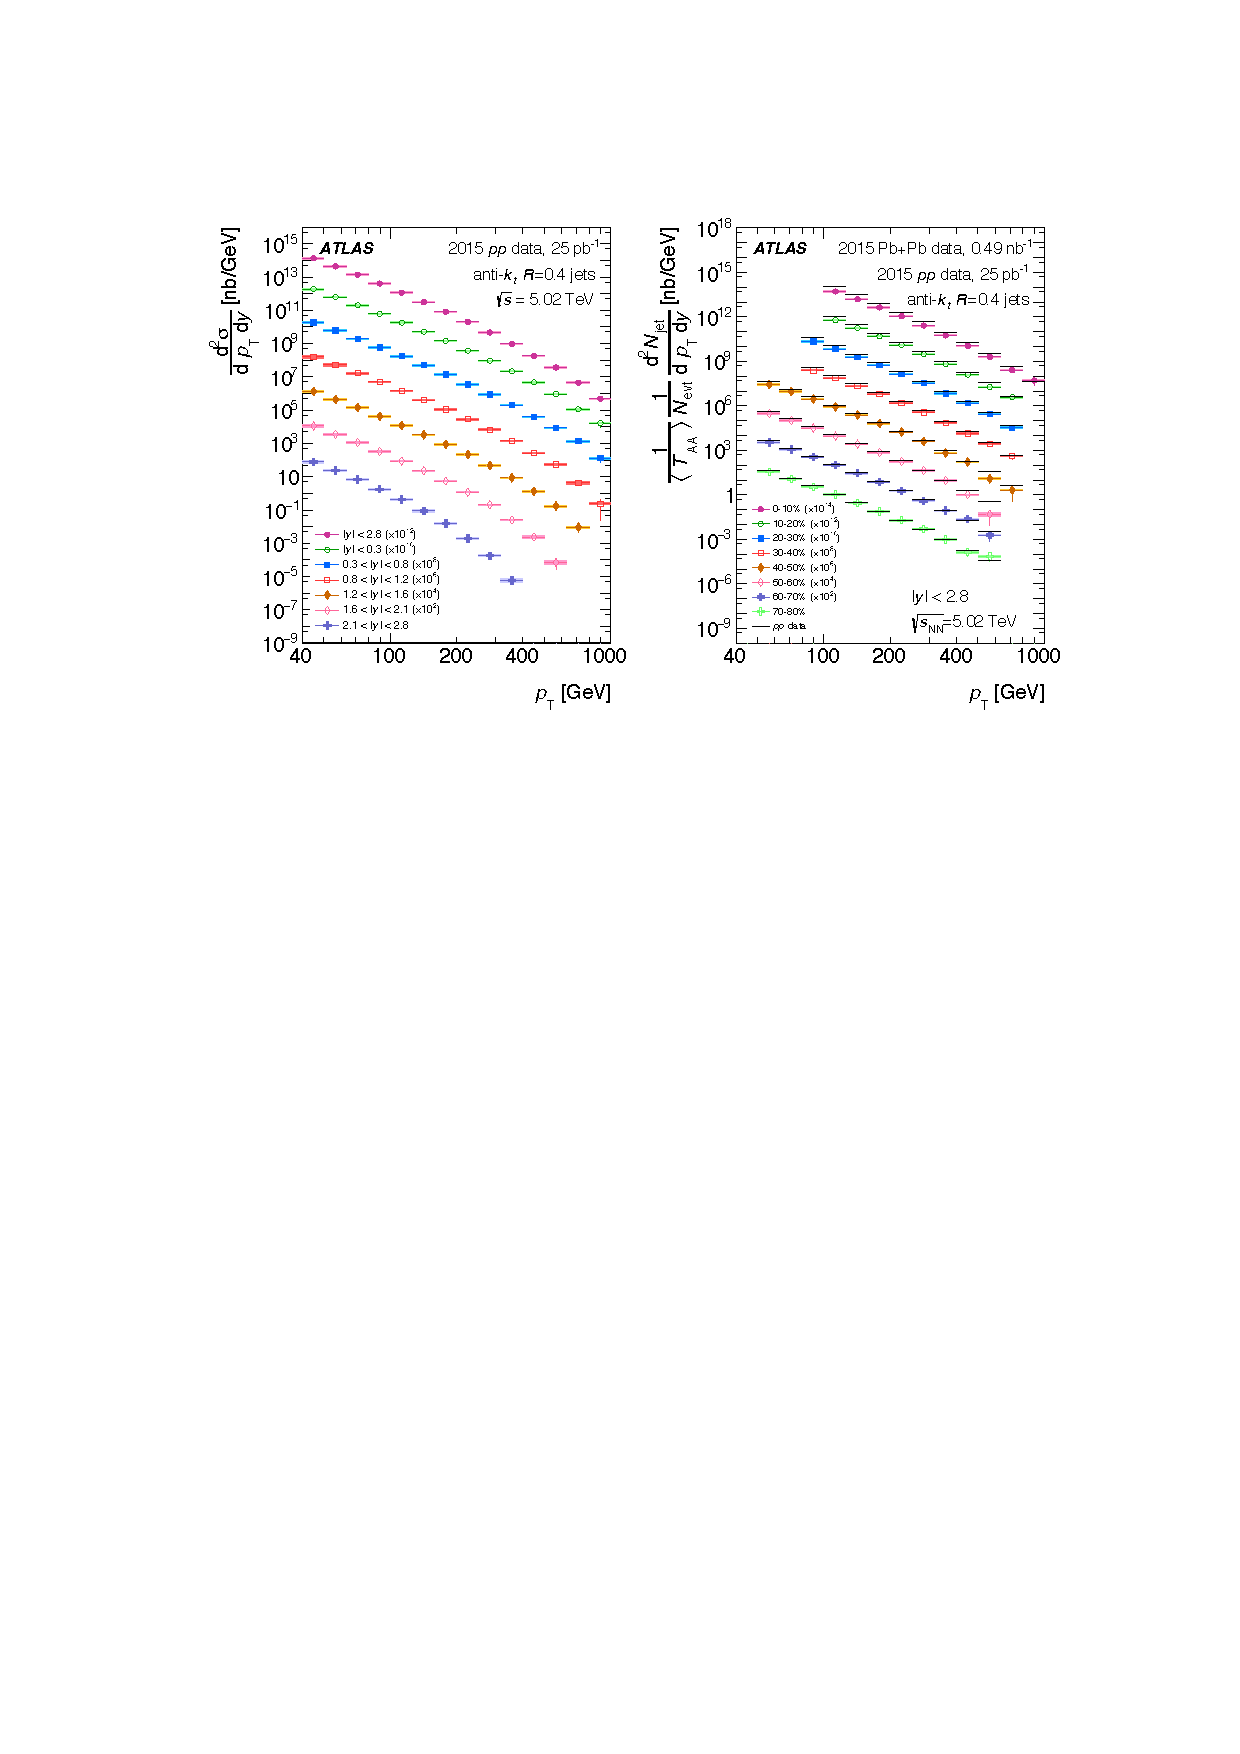
\includegraphics[width=0.85\textwidth]{figures/jetMeasurements/jetYields}
\caption{(Left) The inclusive jet cross section in \pp\ collisions as a function of jet \pt\ in different $|y|$ intervals scaled by successive powers of $10^2$ for visibility. (Right) Per event inclusive jet yield in \pbpb\ collisions normalized by $\langle \TAA \rangle$ as a function of jet \pt\ in different centrality intervals scaled by successive powers of $10^2$ for visibility. The solid lines represent the cross section from \pp\ data at the same rapidity interval scaled by the same $10^2$ factor.  Figure taken from \cite{2019108}}
\label{fig:jet_yields}
\end{center}
\end{figure}


Figure~\ref{fig:raa} shows the measured inclusive jet \RAA\ as a function of jet \pt\ for different centrality bins and jet rapidity $|y| < 2.8$. It can be seen that the most central collisions show a clear suppression with an $\RAA \approx 0.45$ at jet $\pt\ 100$ GeV. The \RAA\ value slowly evolves with jet \pt\ and rises to 0.6 at jet $\pt = 800$ GeV. This modification becomes smaller for more peripheral collisions. 

\begin{figure}[htbp]
\begin{center}
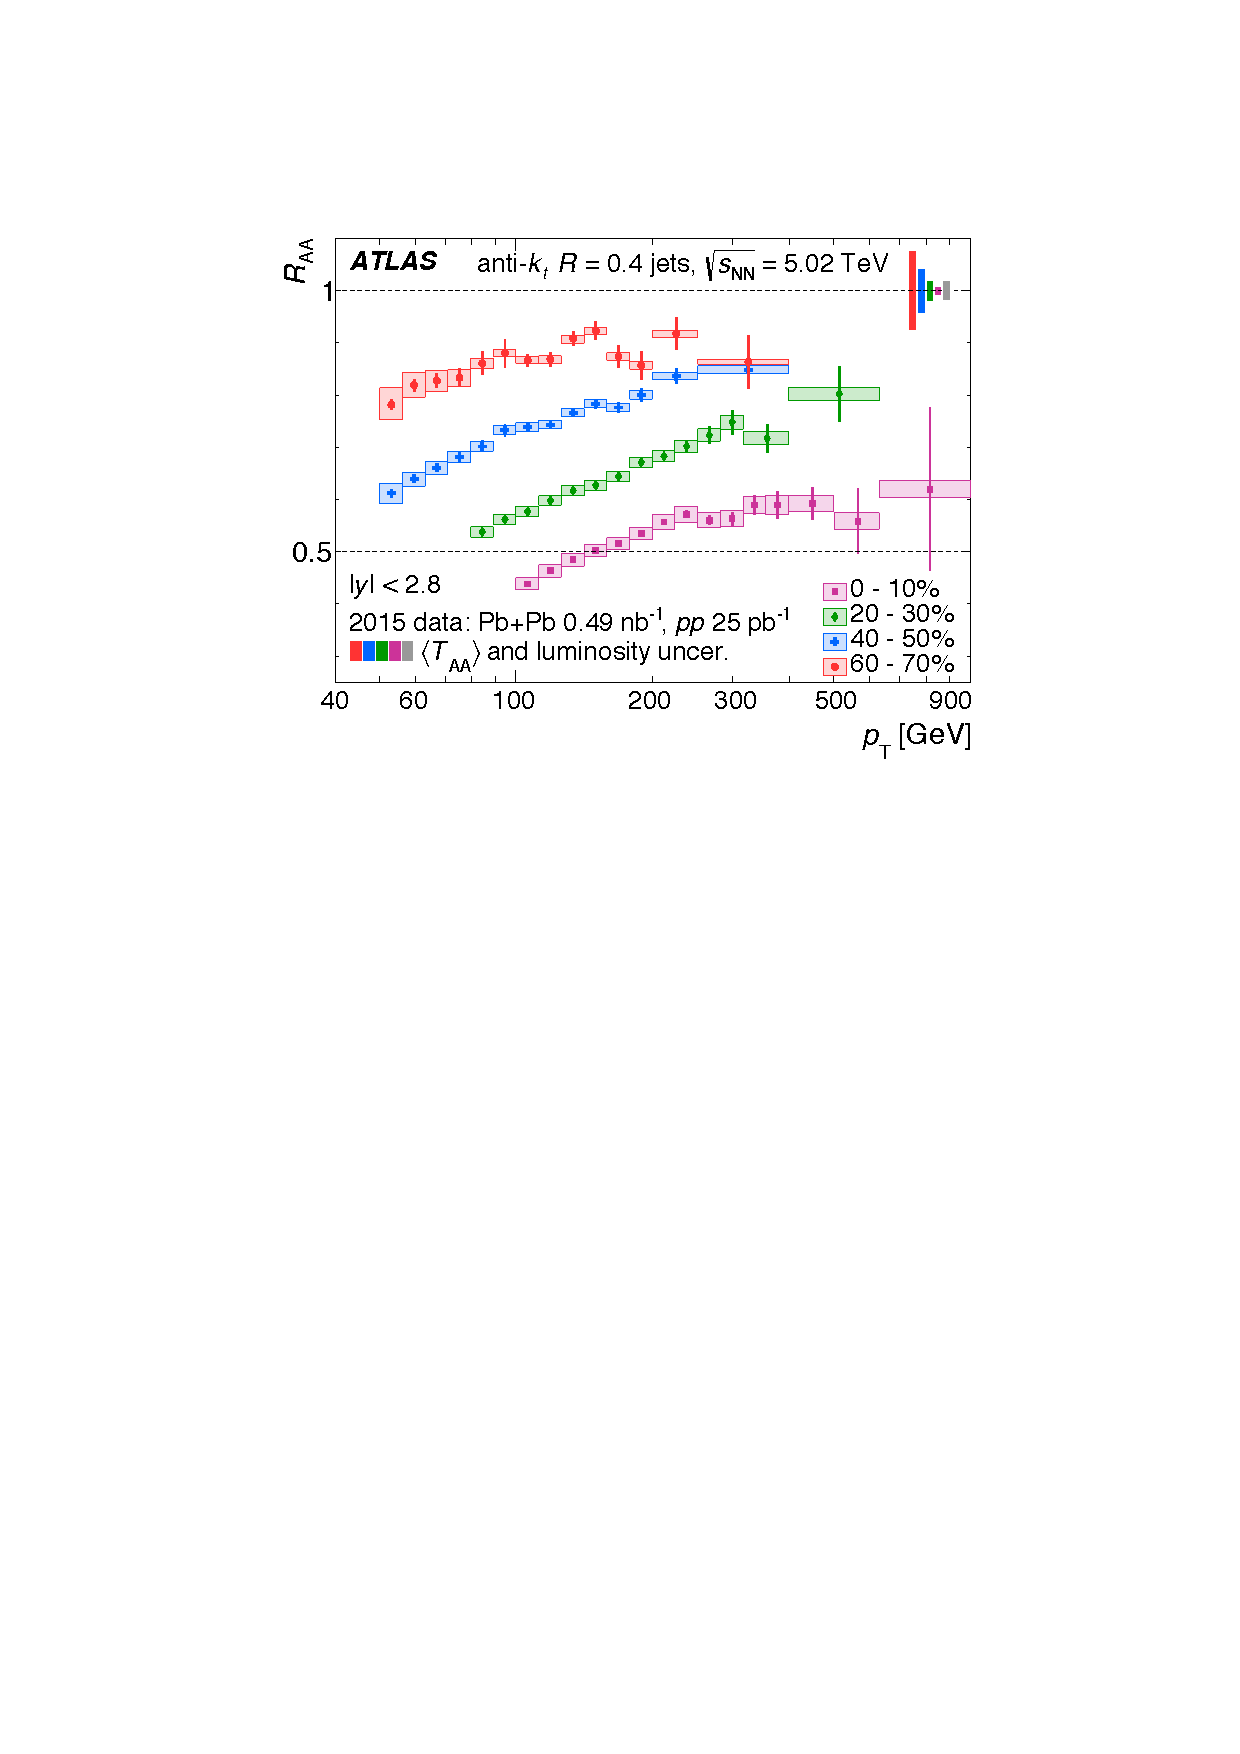
\includegraphics[width=0.55\textwidth]{figures/jetMeasurements/raa}
\caption{The \RAA\ distributions as a function of jet \pt\ for different centrality bins and jet rapidity $|y| < 2.8$. The error bars represent statistical uncertainties while the the shaded boxes represent systematic uncertainties. Figure taken from \cite{2019108}}
\label{fig:raa}
\end{center}
\end{figure}

The smooth centrality dependence can be more clearly seen in Figure~\ref{fig:raa_centDep}, where \RAA\ is shown as a function of \ANpart\ for jets the 100--126 GeV and 200--251 GeV ranges. The magnitude of the suppression is also seen to significantly depend on jet \pt\ for $\ANpart \geq 50$. 

\begin{figure}[htbp]
\begin{center}
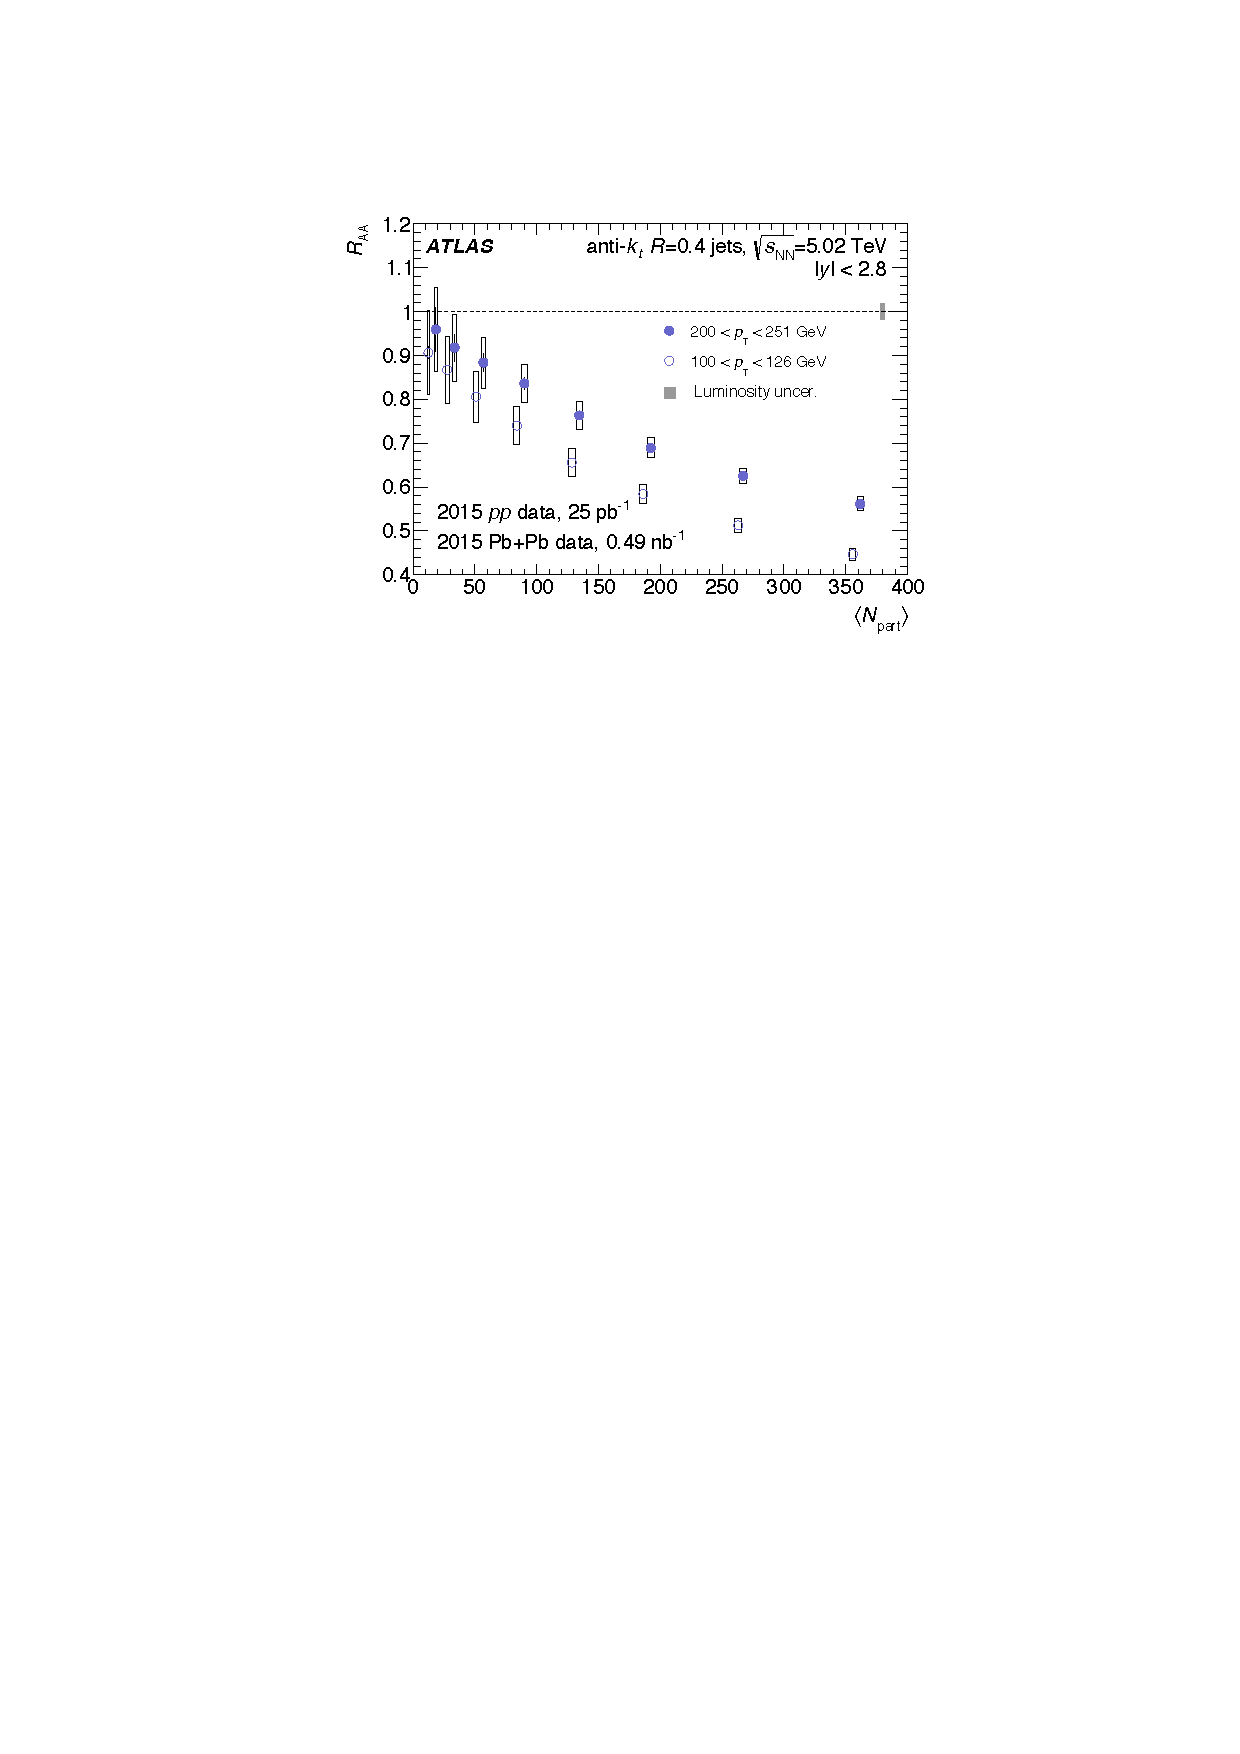
\includegraphics[width=0.55\textwidth]{figures/jetMeasurements/raa_centDep}
\caption{The \RAA\ distributions as a function of jet \pt\ for different centrality bins and jet rapidity $|y| < 2.8$. The error bars represent statistical uncertainties while the the shaded boxes represent systematic uncertainties. Figure taken from \cite{2019108}}
\label{fig:raa_centDep}
\end{center}
\end{figure}

%The measurement further looked at the $y$ dependence of \RAA\ as described by $\RAA (|y|) / \RAA (|y| < 0.3)$. This is useful because it is sensitive to the different quark to gluon fractions at different rapidities.  the uncertainties largely cancel, an













%%%%%%%%%%%%%%%%%%%%%%%%%%%%%%%%%%%%%%
\section{Jet Fragmentation}
\label{sec:jet_ff}
\cite{PhysRevC.98.024908}









%%%%%%%%%%%%%%%%%%%%%%%%%%%%%%%%%%%%%%
\section{Effective Quenching}
This discussion is based on the model introduced in \cite{Spousta:2015fca}. This phenomenological model emphasizes the jet \pt\ dependence of the quark to gluon fraction and the difference between quark-jet and gluon-jet quenching. It uses an ``extended'' power law parameterization of the high-\pt\ hadron spectra coupled with a quenching that is based on a non-constant fractional energy loss. This model considers the different color charges carried by quarks and gluons and their different splitting functions, and assumes that gluon jets lose energy at a rate 9/4 times higher than quark jets. The key assumption of the model are:
\begin{itemize}
\item The energy lost by a jet is radiated at large angles and does not appear within the jet cone. This is backed by \cite{Chatrchyan:2011sx}.
\item The fragmentation pattern of the jet is unaffected by the presence of the QGP i.e. they fragment as they would in a vacuum. This is motivated by the idea that the QGP is unable to resolve the internal jet structure and is supported by \cite{Blaizot:2013hx, CasalderreySolana:2012ef}.
\end{itemize} 

The model uses the following extended power-law parameterization to describe the high-\pt\ jet spectra:

\begin{align}
\frac{dn}{d\ptjet} = A \left( \frac{\pt_0}{\ptjet} \right) ^{n+\beta \log(\ptjet / \pt_0)}
\end{align}

where $\pt_0$ is a reference transverse momentum at which $A= dn/d\ptjet$, $\beta$ is the logarithmic derivative of $dn/d\ptjet$ at $\ptjet = \pt_0$. Then considering the different quark and gluon fractions as $f_{q0}$ and $f_{g0} = 1-f_{q0}$ respectively, the combined spectrum for quarks and gluons can be written as:

\begin{align}
 \frac{dN}{d\ptjet} &= A \left[ f_{q0} \left( \frac{\pt_0}{\ptjet} \right)^{n_q+ \beta_q \log(\ptjet / \pt_0)} + (1-f_{q0}) \left( \frac{\pt_0}{\ptjet} \right)^{n_g + \beta_g \log(\ptjet / \pt_0)} \right] \\
\nonumber \\ 
\label{eq:eq_q_frac} f_q (\ptjet) &= \dfrac{1}{1 + \left(\dfrac{1-f_{q0}}{f_{q0}}\right) \left( \dfrac{\pt_0}{\ptjet}\right)^{\Delta n + \Delta \beta \log(\ptjet/\pt_0)} }
\end{align}
where $\Delta n = n_g - n_q$ and $\Delta \beta = \beta_g - \beta_q$. The \pt\ dependence of the quark fraction along with the fit is shown in Figure~\ref{fig:raa_centDep}. The fragmentation functions can also be determined using final-state charged hadrons within a $R=0.4$ jet cone. These are fit to the form \Dz, with fits for the quark and gluon fragmentation shown in Figure~\ref{fig:gluon_fragmentation}.


\begin{align}
D(z) = a \times \frac{(1+dz)^b}{(1+ez)^c} \times e^{-fz}
\label{eq:ff_param}
\end{align}


\begin{figure}
\begin{subfigure}{.45\textwidth}
  \centering
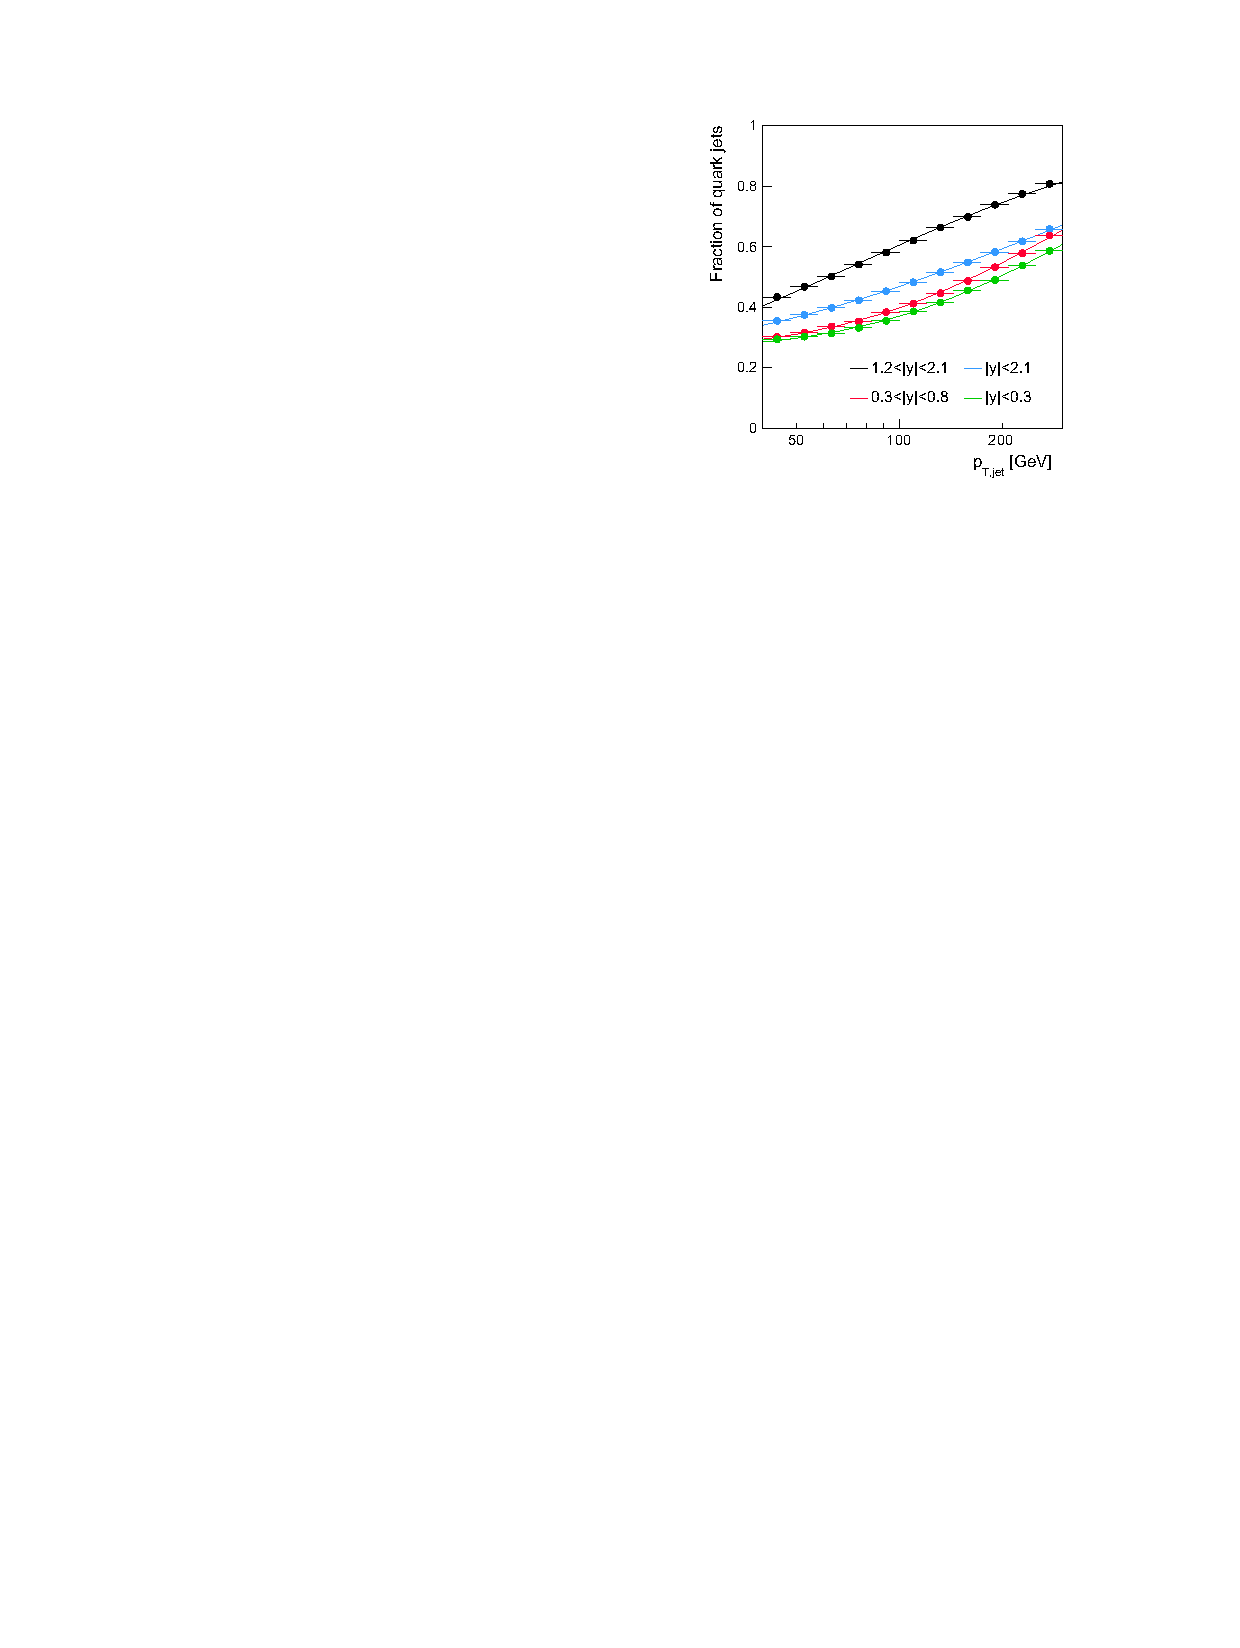
\includegraphics[width=0.8\textwidth]{figures/jetMeasurements/jetQuarkFraction}
\caption{The jet quark fraction as a function of \ptjet\ in different rapidity bins. The points are from \pythia8 simulations and the lines are fits to Equation~\ref{eq:eq_q_frac}.}
\label{fig:raa_centDep}
\end{subfigure} \qquad
\begin{subfigure}{.45\textwidth}
  \centering
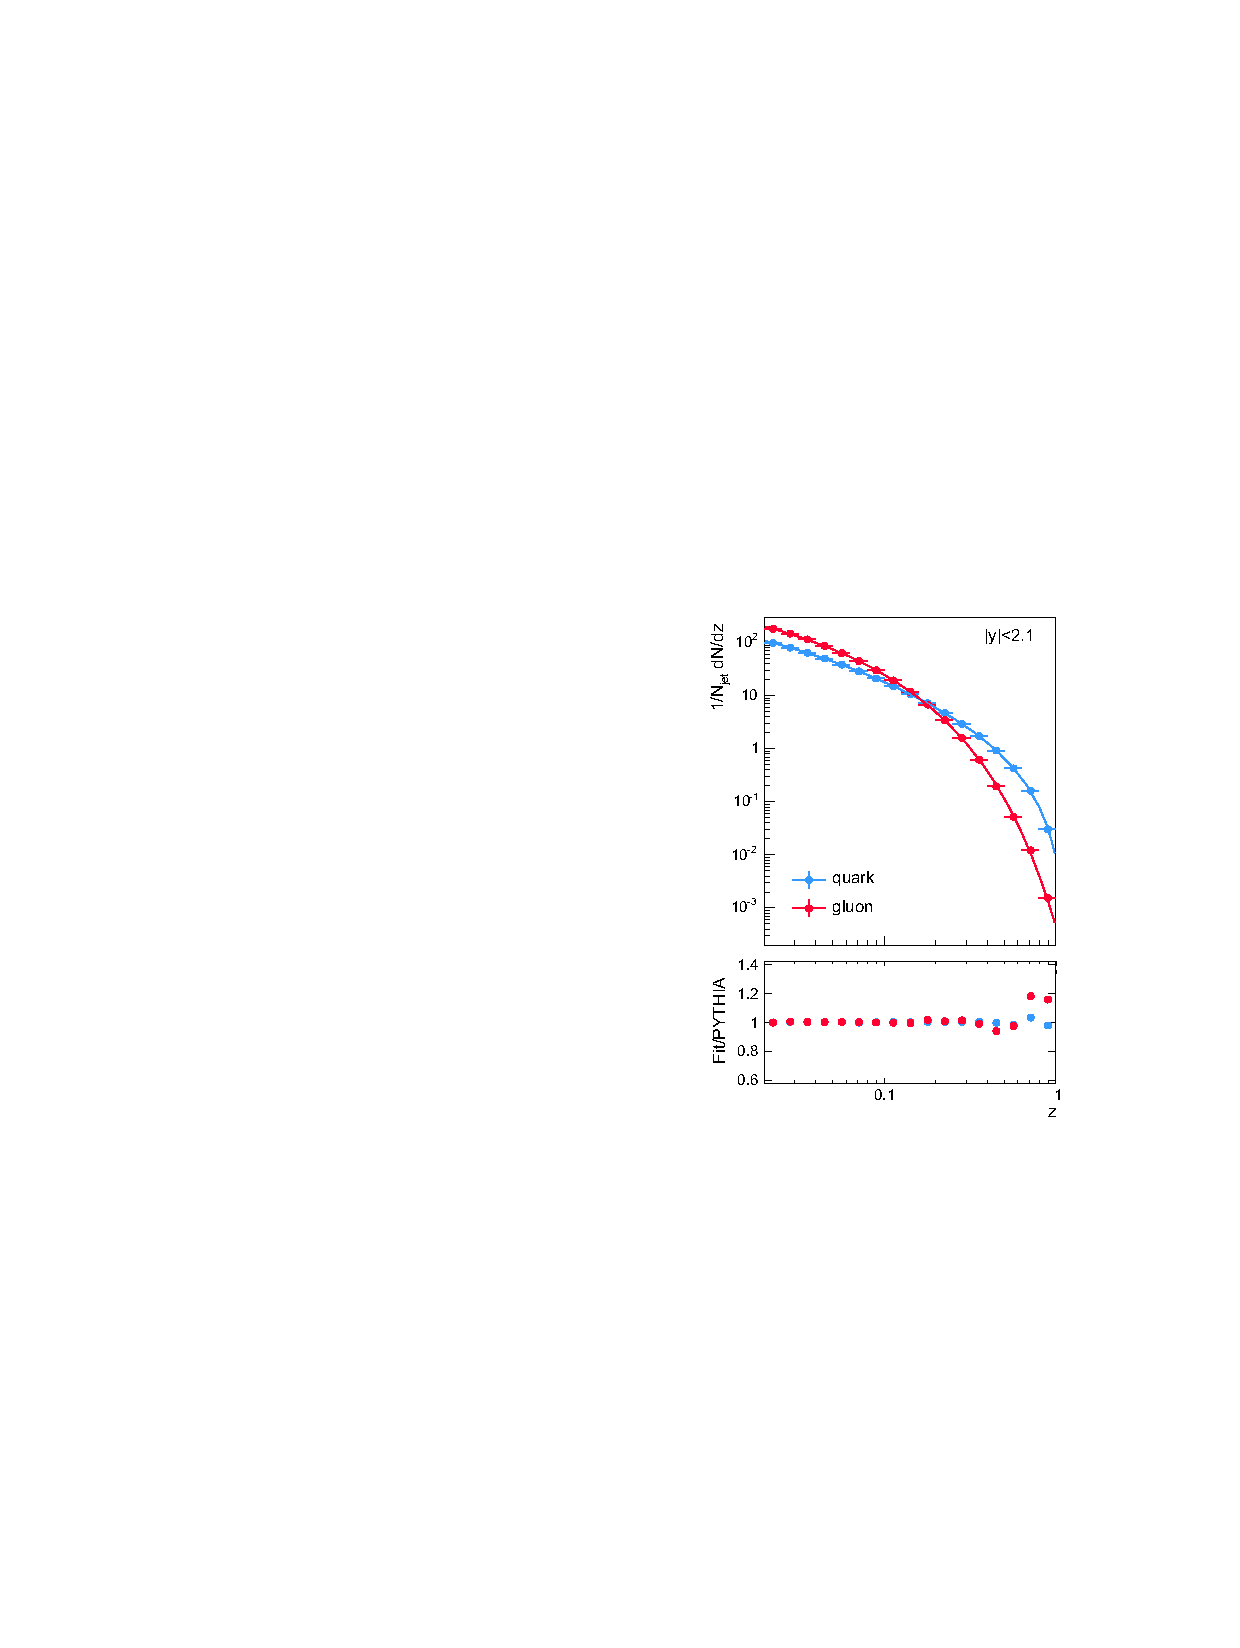
\includegraphics[width=0.8\textwidth]{figures/jetMeasurements/gluon_fragmentation}
\caption{A comparison of the \pythia8 quark and gluon fragmentation. The solid lines are the fits from The jet quark fraction as a function of \ptjet\ in different rapidity bins. The points are from \pythia8 simulations and the lines are fits to Equation~\ref{eq:ff_param}.}
\label{fig:gluon_fragmentation}
\end{subfigure}
\caption{Fits to quark fractions and fragmentation functions from \pythia8.  Figure taken from \cite{Spousta:2015fca}}
\label{fig:EQ_pp_models}
\end{figure}


For the quenched spectra, this model assumes a non-constant fractional shift given below as $S$. This approach is based on \cite{baier2001quenching} and is used because of the inability of the constant fractional shift to explain the jet \pt\ dependence of measured \RAA. 

\begin{align}
S = s' \left( \frac{\ptjet}{\pt_0} \right) ^\alpha
\end{align}
where $\alpha$ is an undetermined parameter and $s'$ is the shift for a jet with $\ptjet = \pt_0$. This gives the following quenched high-\pt\ hadron spectra:

\begin{align}
 \frac{dN_Q}{d\ptjet} &= A \Bigg[ f_{q0} \left( \frac{\pt_0}{\ptjet+S_q} \right)^{n_q+ \beta_q \log\big((\ptjet+S_q) / \pt_0\big)} \left(1 + \frac{dS_q}{d\ptjet} \right) \\
& + (1-f_{q0}) \left( \frac{\pt_0}{\ptjet+S_g} \right)^{n_g + \beta_g \log\big((\ptjet+S_g) / \pt_0\big)}  \left(1 + \frac{dS_g}{d\ptjet} \right) \Bigg] \nonumber
\end{align}
Where the $(1+dS/d\ptjet)$ term is a Jacobian to preserve the number of jets. 
Then the \RAA\ can be written as:

\begin{align}
\RAA = f_q & \left(\frac{1}{1 + S_q / \ptjet}\right) ^{n_q + \beta_q \log\big((\ptjet+S_q)/\pt_0\big)}  \frac{\pt_0}{\ptjet}^{} \left( 1+ \frac{dS_q}{d\ptjet} \right) \times  \\
 (1-f_q) & \left(\frac{1}{1 + S_g / \ptjet}\right) ^{n_g + \beta_g \log\big((\ptjet+S_g)/\pt_0\big)}  \frac{\pt_0}{\ptjet}^{} \left( 1+ \frac{dS_g}{d\ptjet} \right)  \nonumber \\
\end{align}
where the flavor fraction is given by Equation~\ref{eq:eq_q_frac}. These can be fit to the measured ATLAS \RAA\ data as shown in Figure~\ref{fig:EQ_RAA} and the parameters $s'$ and $\alpha$ can be extracted as shown in Figure~\ref{fig:eq_param}. 

\begin{figure}[htbp]
\begin{center}
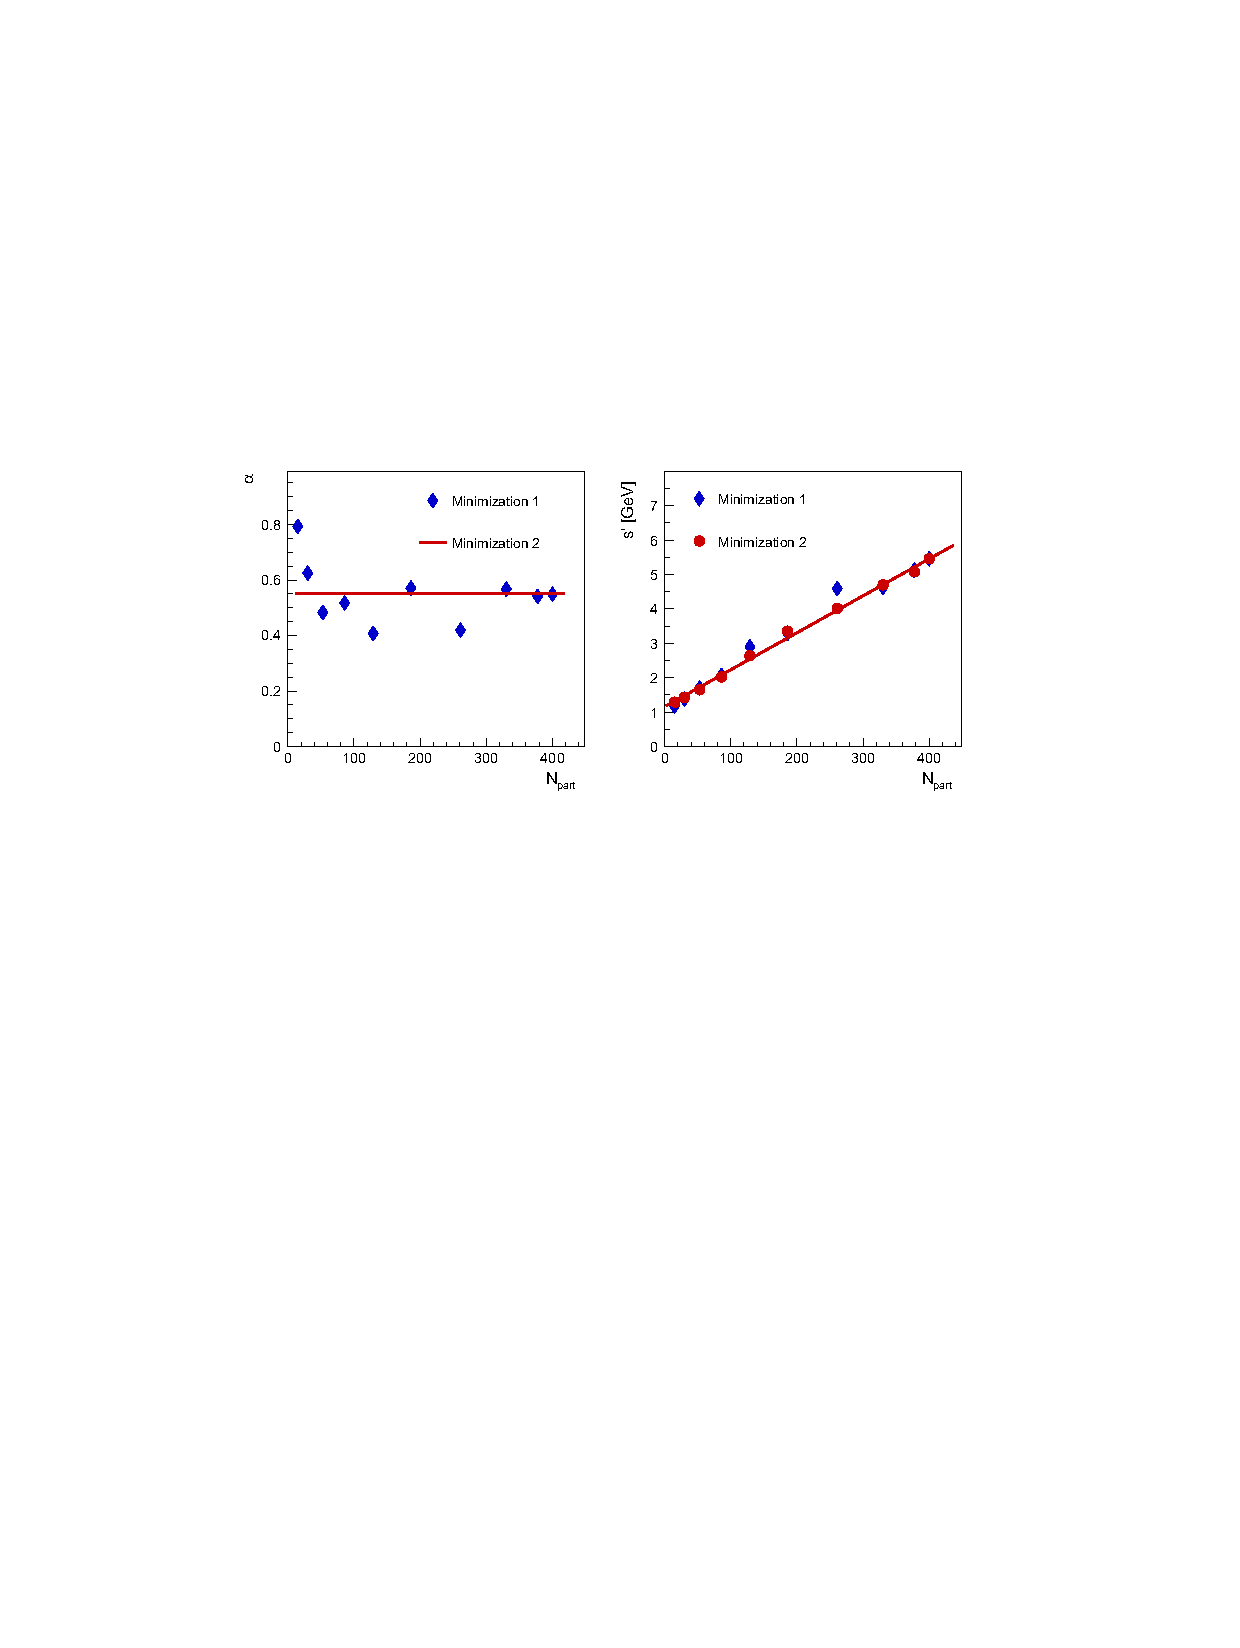
\includegraphics[width=0.55\textwidth]{figures/jetMeasurements/EQ_fitQuality}
\caption{The extracted values of $\alpha$ and $s'$ as a function of \Npart. The first minimization shows fluctuations for $\alpha$ around 0.55, which was then fixed for the second minimization to give an $s'$ that linearly depends on \Npart. Figure taken from \cite{Spousta:2015fca}}
\label{fig:eq_param}
\end{center}
\end{figure}

It can be seen that the analytic fits and the MC are in good agreement. While the fits agree with the data by definition, the robustness of the model can be seen in that it describes the data with a single value for $\alpha$ and a simple centrality dependent shift constant $s'$.  Fits to the \Dz\ distributions are shown in Figure~\ref{fig:EQ_FF} and it can be seen that while the MC and analytic calculation agree well with each other, they are only able to qualitatively capture some features of the data. The enhancement at high $z$ can be explained by an increased quark content of the jet spectrum and subsequent differential quenching for quark and gluon jets. The low $z$ enhancement on the other hand can be considered to be a result of a gluon radiation within the jet or a wake from the medium itself.

\begin{figure}
\begin{subfigure}{1\textwidth}
  \centering
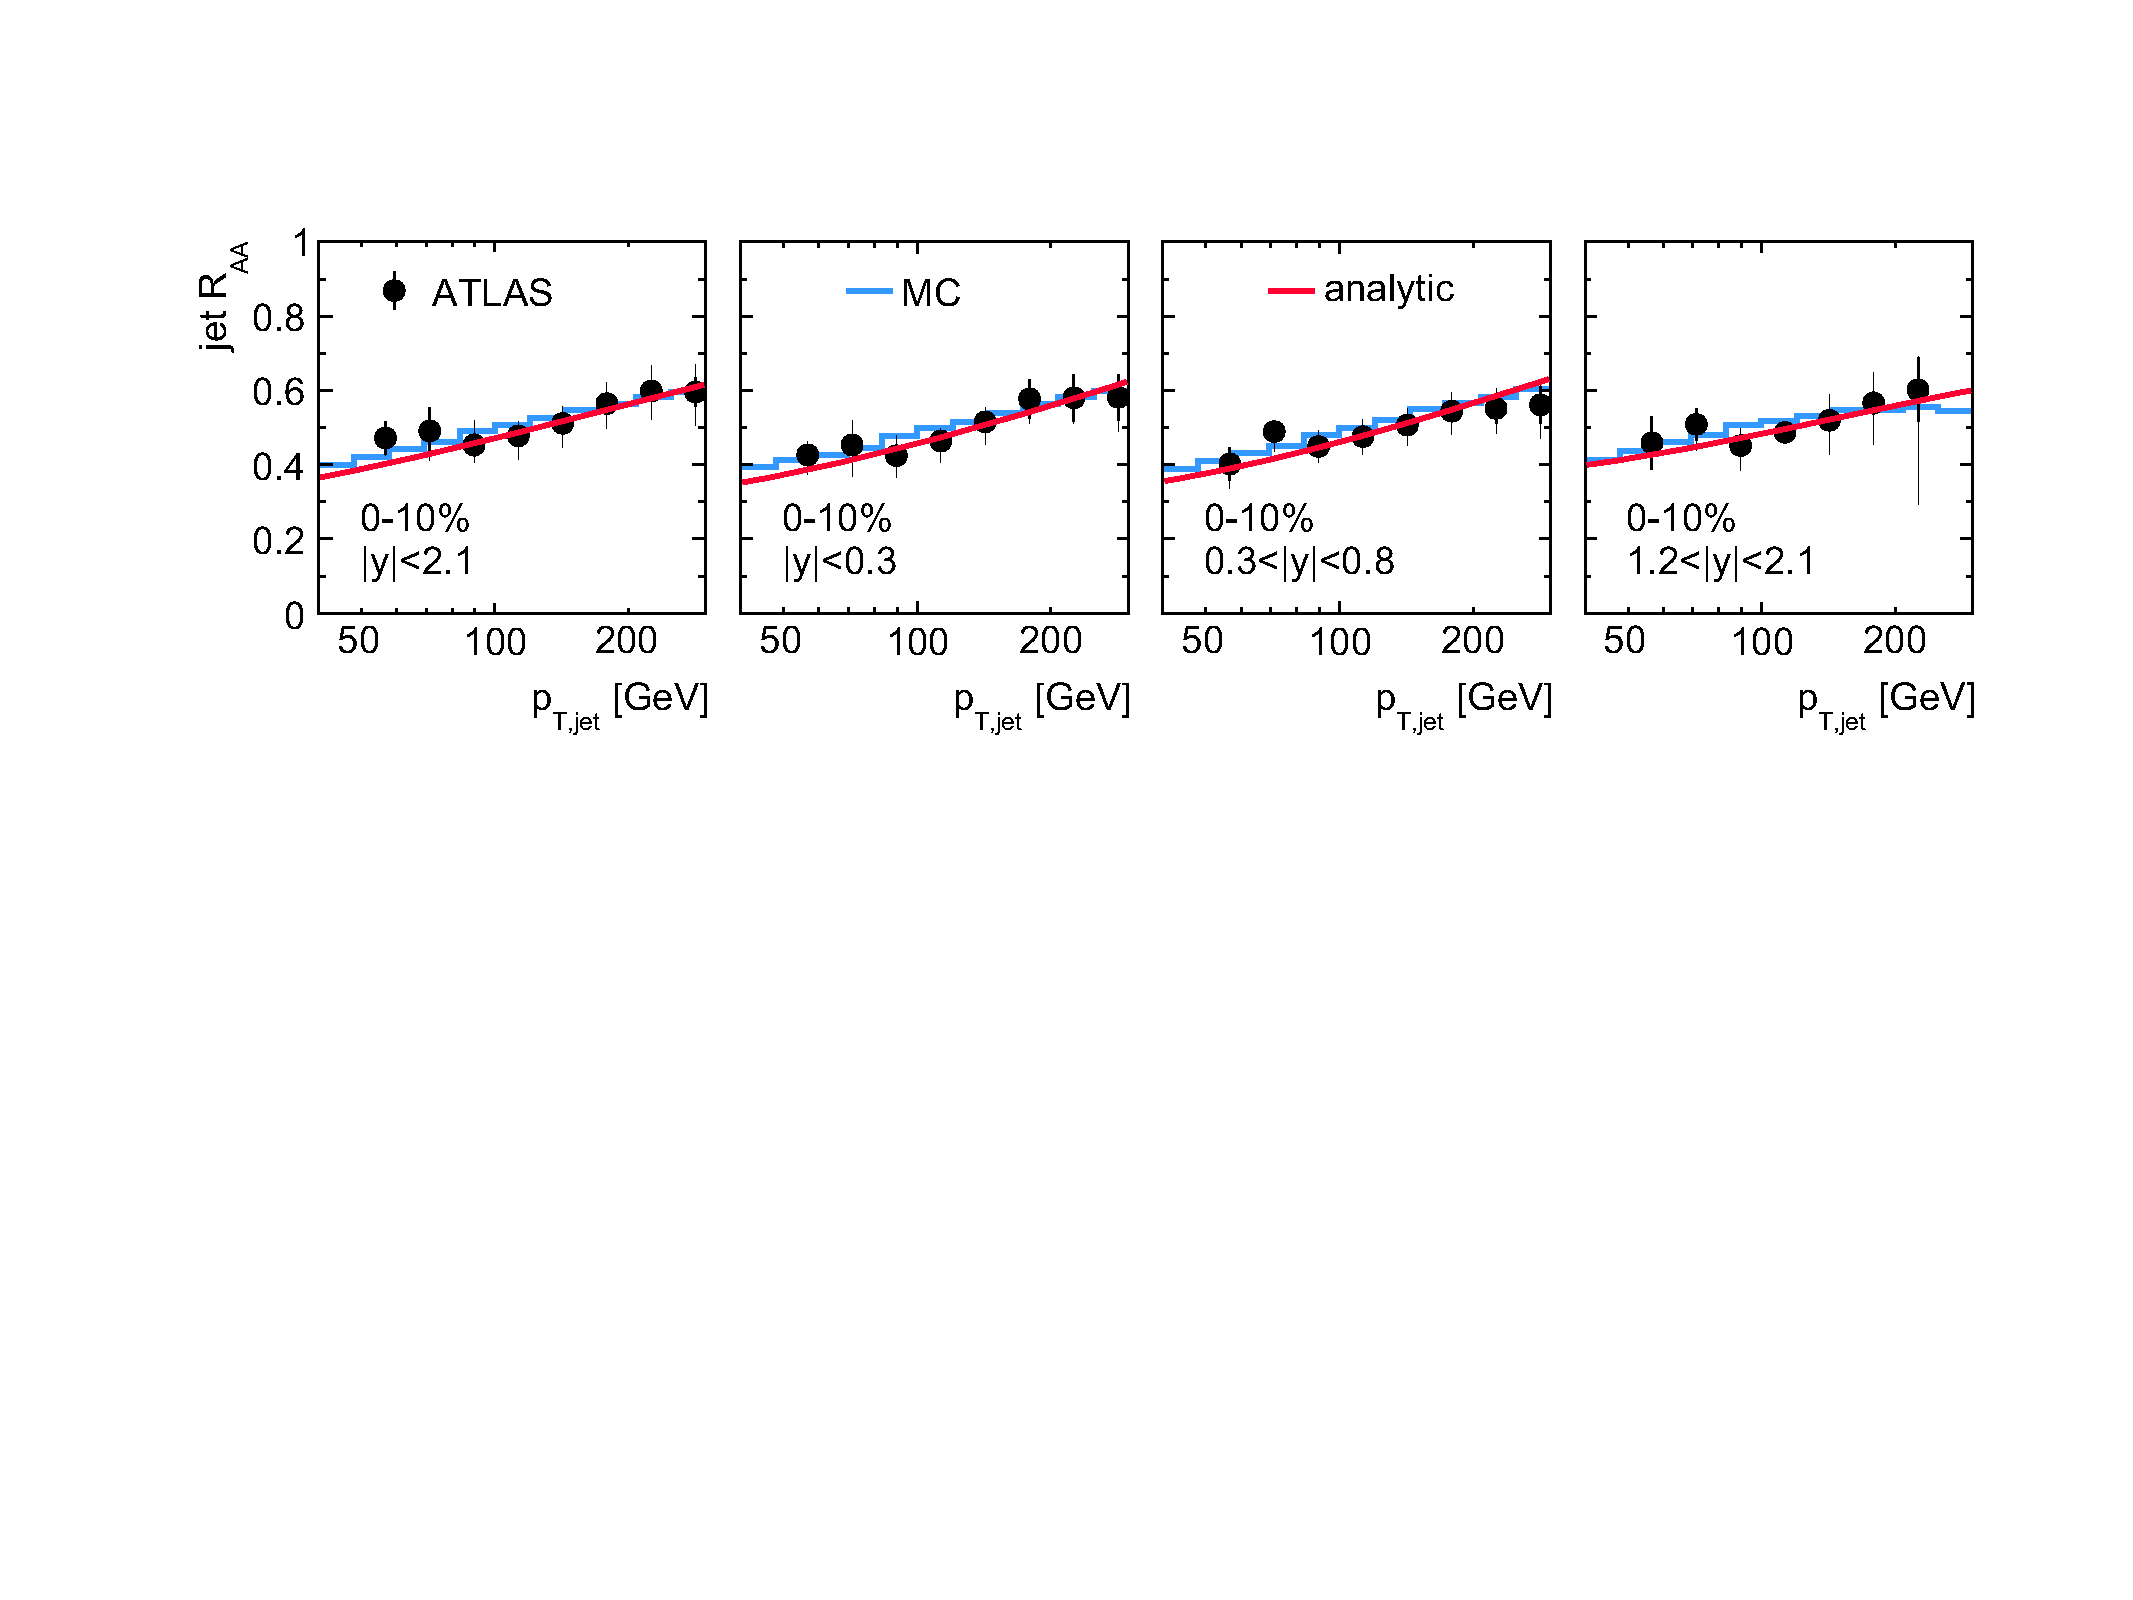
\includegraphics[width=1\textwidth]{figures/jetMeasurements/EQ_RAA}
\caption{A comparison of the \RAA\ as measured by ATLAS for central \pbpb\ collisions in \cite{Aad:2014bxa}, a MC calculation (blue) and the analytic calculation (red) in the EQ model with the extended power-law parameterization and a non-constant fractional energy loss. The different panels are different rapidity intervals.}
\label{fig:EQ_RAA}
\end{subfigure} \\ \\ \\
\begin{subfigure}{1\textwidth}
  \centering
\includegraphics[width=1\textwidth]{figures/jetMeasurements/eq_FF}
\caption{A comparison of the \Rdz\ as measured by ATLAS in \cite{Aad:2014wha}, a MC calculation (blue) and the analytic calculation (red) in the EQ model with the extended power-law parameterization and a non-constant fractional energy loss. The different panels are different centrality intervals.}
\label{fig:EQ_FF}
\end{subfigure}
\caption{A comparison of measured data, MC, and the analytic calculation of the EQ model. Figure taken from \cite{Spousta:2015fca}}
\label{fig:EQ_modification}
\end{figure}




%%%%%%%%%%%%%%%%%%%%%%%%%%%%%%%%%%%%%%
\subsection{Jet Fluid model}
This discussion is based on the model introduced in \cite{Tachibana:2017syd}. This model is based on the evolution of the jet and QGP in a coupled manner, considering the energy and transverse momentum exchange between them. In this picture, both the jet and medium are allowed to modify each other; the jet is modified via collisional and radiative processes while the medium evolves hydrodynamically and is modified because it picks up the energy lost by the jet. 

The time evolution of the jet is given 

\begin{align}
f_i (\omega_i, \kTsq_i, t) = \frac{dN_i (\omega_i \kTsq_i, t)}{d \omega_i d\kTsq_i}
\end{align}
where $i$ is the type of parton, $\omega_i$ is its energy, and $\kTsq$ is its transverse momentum with respect to the jet axis. Then the transport equations can be written in terms of :

\begin{align}
\label{eq:jf_transportEq}
\frac{d f_j}{dt} &= \hat{e_j} \frac{\p f_j}{\p \omega_j} + \frac{1}{4} \hat{q_j} \nabla_{\kT}^2 f_j  \\
& + \sum_i \int d\omega_i d\kTsq_i \frac{d\widetilde{\Gamma}_{i\rightarrow j} }{d\omega_j d\kTsq_j dt} f_i \\
& - \sum_i \int d\omega_i d\kTsq_i \frac{d\widetilde{\Gamma}_{j\rightarrow i} }{d\omega_ij d\kTsq_i dt} f_i \\
\end{align}
where the first term is the collisional energy loss, the second term is the transverse momentum broadening, and the last two terms are the medium induced gain and loss radiative processes respectively. The splitting processes are are given by:

\begin{align}
\frac{d\Gamma_{i \rightarrow j}}{d \omega_j d\kTsq_j dt} = \frac{2\alpha_S}{\pi} \hat{q}_g \frac{x P_{i \rightarrow j} (x)}{\omega_j {k_{\rm T}^4}_j} \sin^2 \left(\dfrac{t - t_i}{2\tau_f} \right)
\end{align}
where $P_{i \rightarrow j} $ is the vacuum splitting function for $i \rightarrow j $ with $\omega_j$ being the energy of the radiated parton, $\tau_f$ is the formation time of the radiated parton, and $\kT_j$ is the transverse momentum of the radiated parton with respect to the parent parton. These transport Equations~\ref{eq:jf_transportEq} can be solved numerically and agree with \RAA\ measurements \cite{Aad:2014bxa, Khachatryan:2016jfl, Abelev:2013kqa}. The effects of the medium are included by considering the energy-momentum conservation of the jet-QGP system $ \p_\mu [T_{\rm QGP}^{\mu\nu} + T_{\rm jet}^{\mu\nu}] = 0$. Then the source term $J^\nu(x)$ that describes the energy transfer between the jet and the medium can be defined as $J^\nu(x) \equiv -\p_\mu  T_{\rm jet}^{\mu\nu}$, making the QGP evolution being given by

\begin{align}
 \p_\mu T_{\rm QGP}^{\mu\nu} = j^\nu
\end{align}
which characterizes the energy-momentum transfer between the jet and the QGP. 

An. important component of this model is the flow induced by jets. A snapshot of this is shown in Figure~\ref{fig:jf_snapshot}, where the evolution of the energy density of the medium can be seen in a sample event. A single jet travels through the QGP, and can be clearly seen in the lower panels after the energy of the medium has been subtracted out. The V shaped feature seen is the mach cone that is induced by the parton as it moves faster than the medium sound velocity. 

\begin{figure}[htbp]
\begin{center}
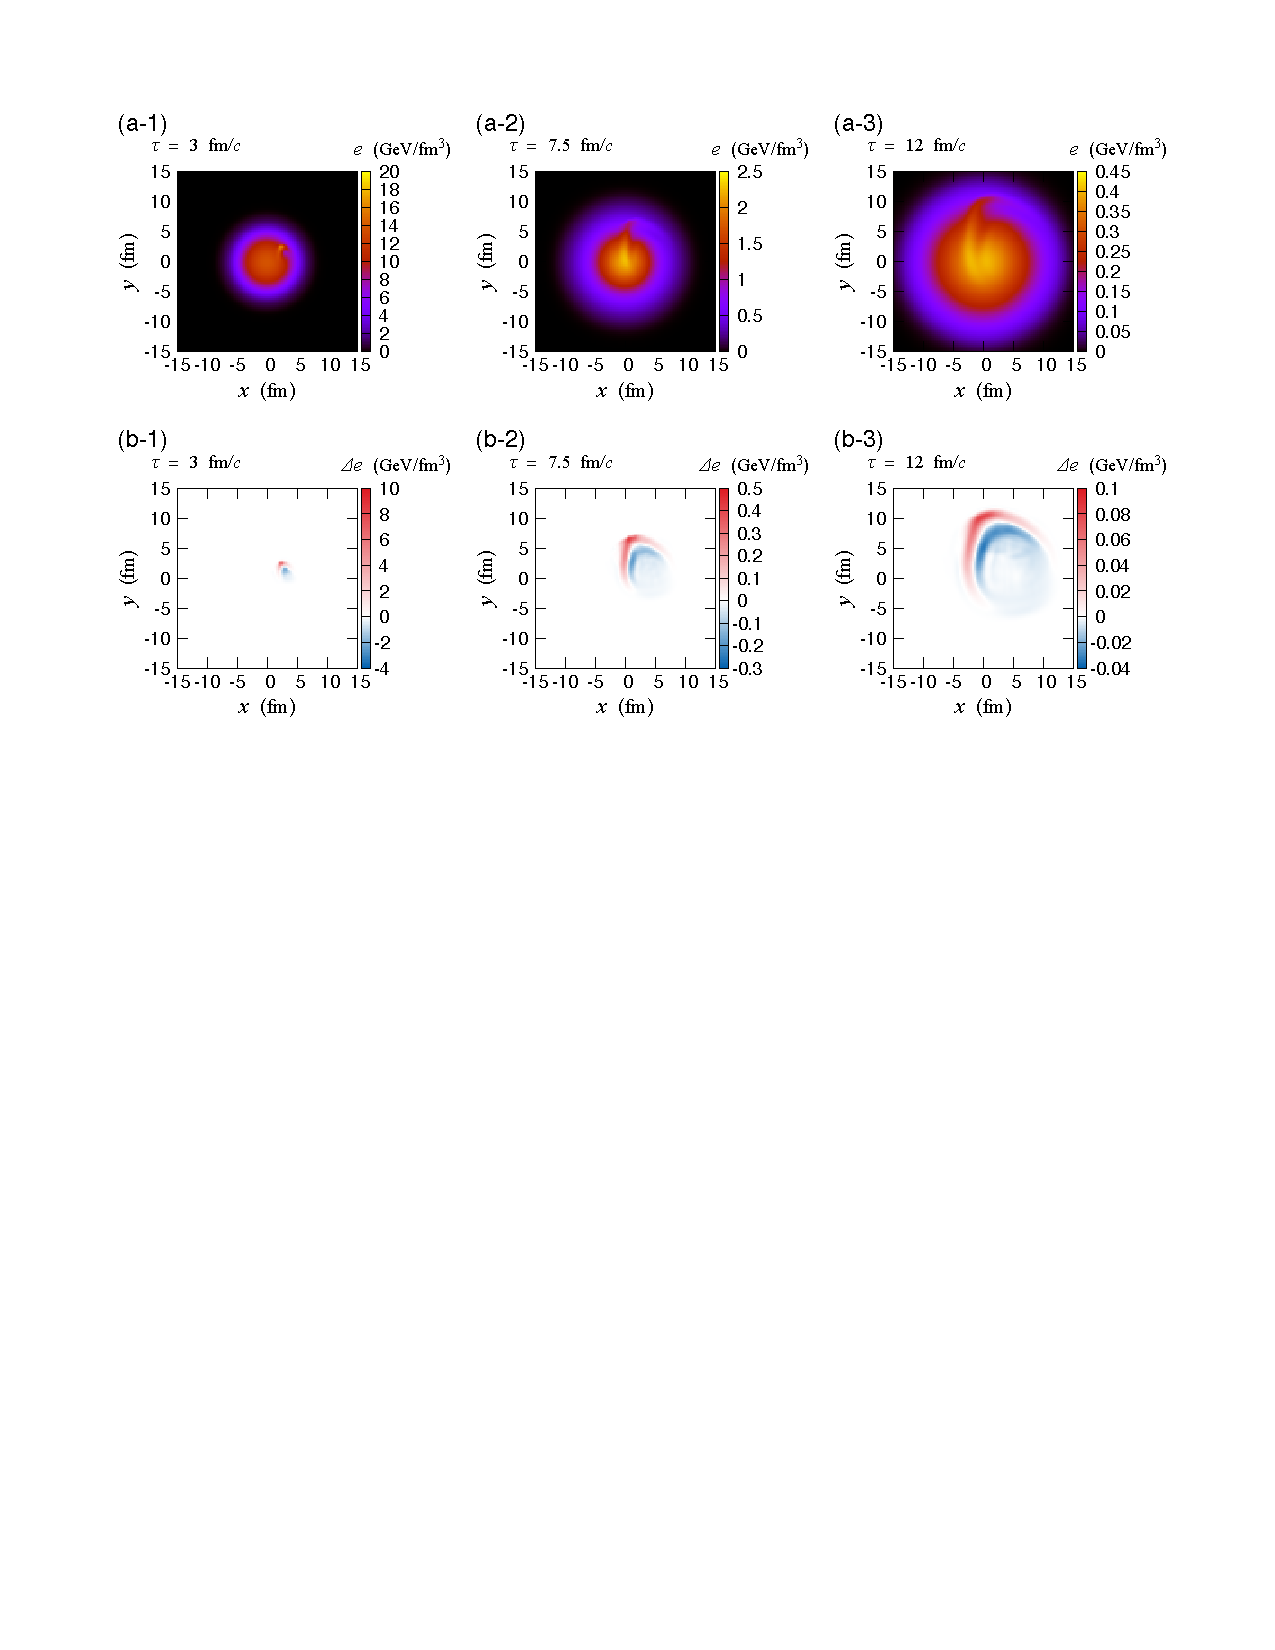
\includegraphics[width=0.85\textwidth]{figures/jetMeasurements/JF_snapshot}
\caption{(Top) The time evolution of the energy density of the quark gluon plasma with a jet propagating through it. (Bottom) The time evolution of the energy density in the event after the energy density of the QGP has been subtracted out. Figure taken from \cite{Tachibana:2017syd}.}
\label{fig:jf_snapshot}
\end{center}
\end{figure}

The final jet energy has two components: the jet shower, and the hydrodynamic response. The former as discussed above comprises of the collisional energy loss, momentum broadening, and medium induced radiation. The latter includes the energy lost from the jet shower that thermalizes into the medium and induces conical flow, some of which is still in the jet cone. This compensates some of the energy lost in the shower and can be seen in Figure~\ref{fig:jf_energyLoss}. While the absolute amount of energy lost increases as a function of initial jet energy, the fractional energy loss decreases. Furthermore there is a cone size dependence once the hydrodynamic contributions are included. This is a result of the jet being highly collimated, such that while an increase in the size does not change the energy much, it does affect the hydrodynamic contribution from the medium.
\begin{figure}[htbp]
\begin{center}
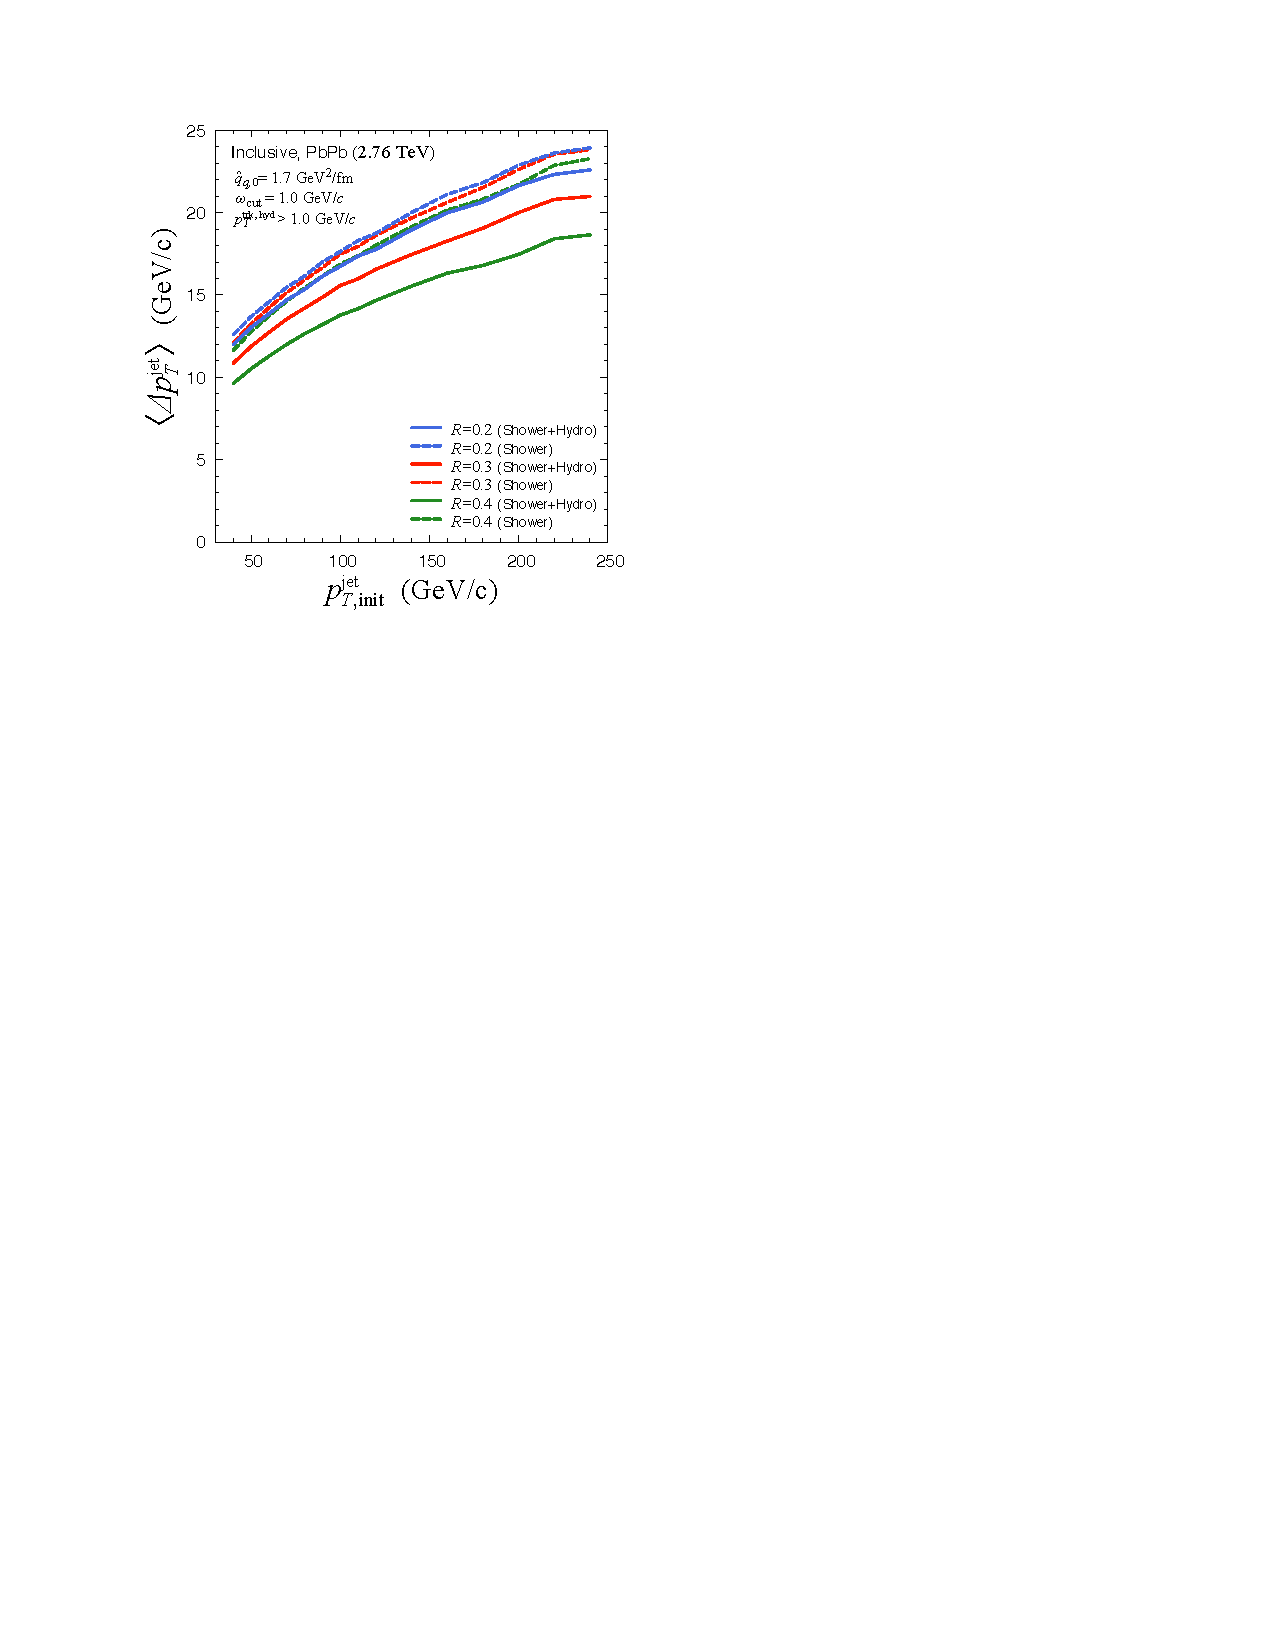
\includegraphics[width=0.45\textwidth]{figures/jetMeasurements/JF_energyLoss}
\caption{(Top) The energy lost by a jets of different radii as a function of their initial energy in central \pbpb\ collisions at \sqrtsnn = 2.76 TeV. Figure taken from \cite{Tachibana:2017syd}.}
\label{fig:jf_energyLoss}
\end{center}
\end{figure}

The \RAA\ distributions constructed with this model and compared to data from CMS \cite{Khachatryan:2016jfl} are shown in Figure~\ref{fig:jf_raa}. Including the hydrodynamic contribution decreases the energy loss, hence increasing the \RAA\ value and inducing a cone size dependence to the \RAA. 

\begin{figure}[htbp]
\begin{center}
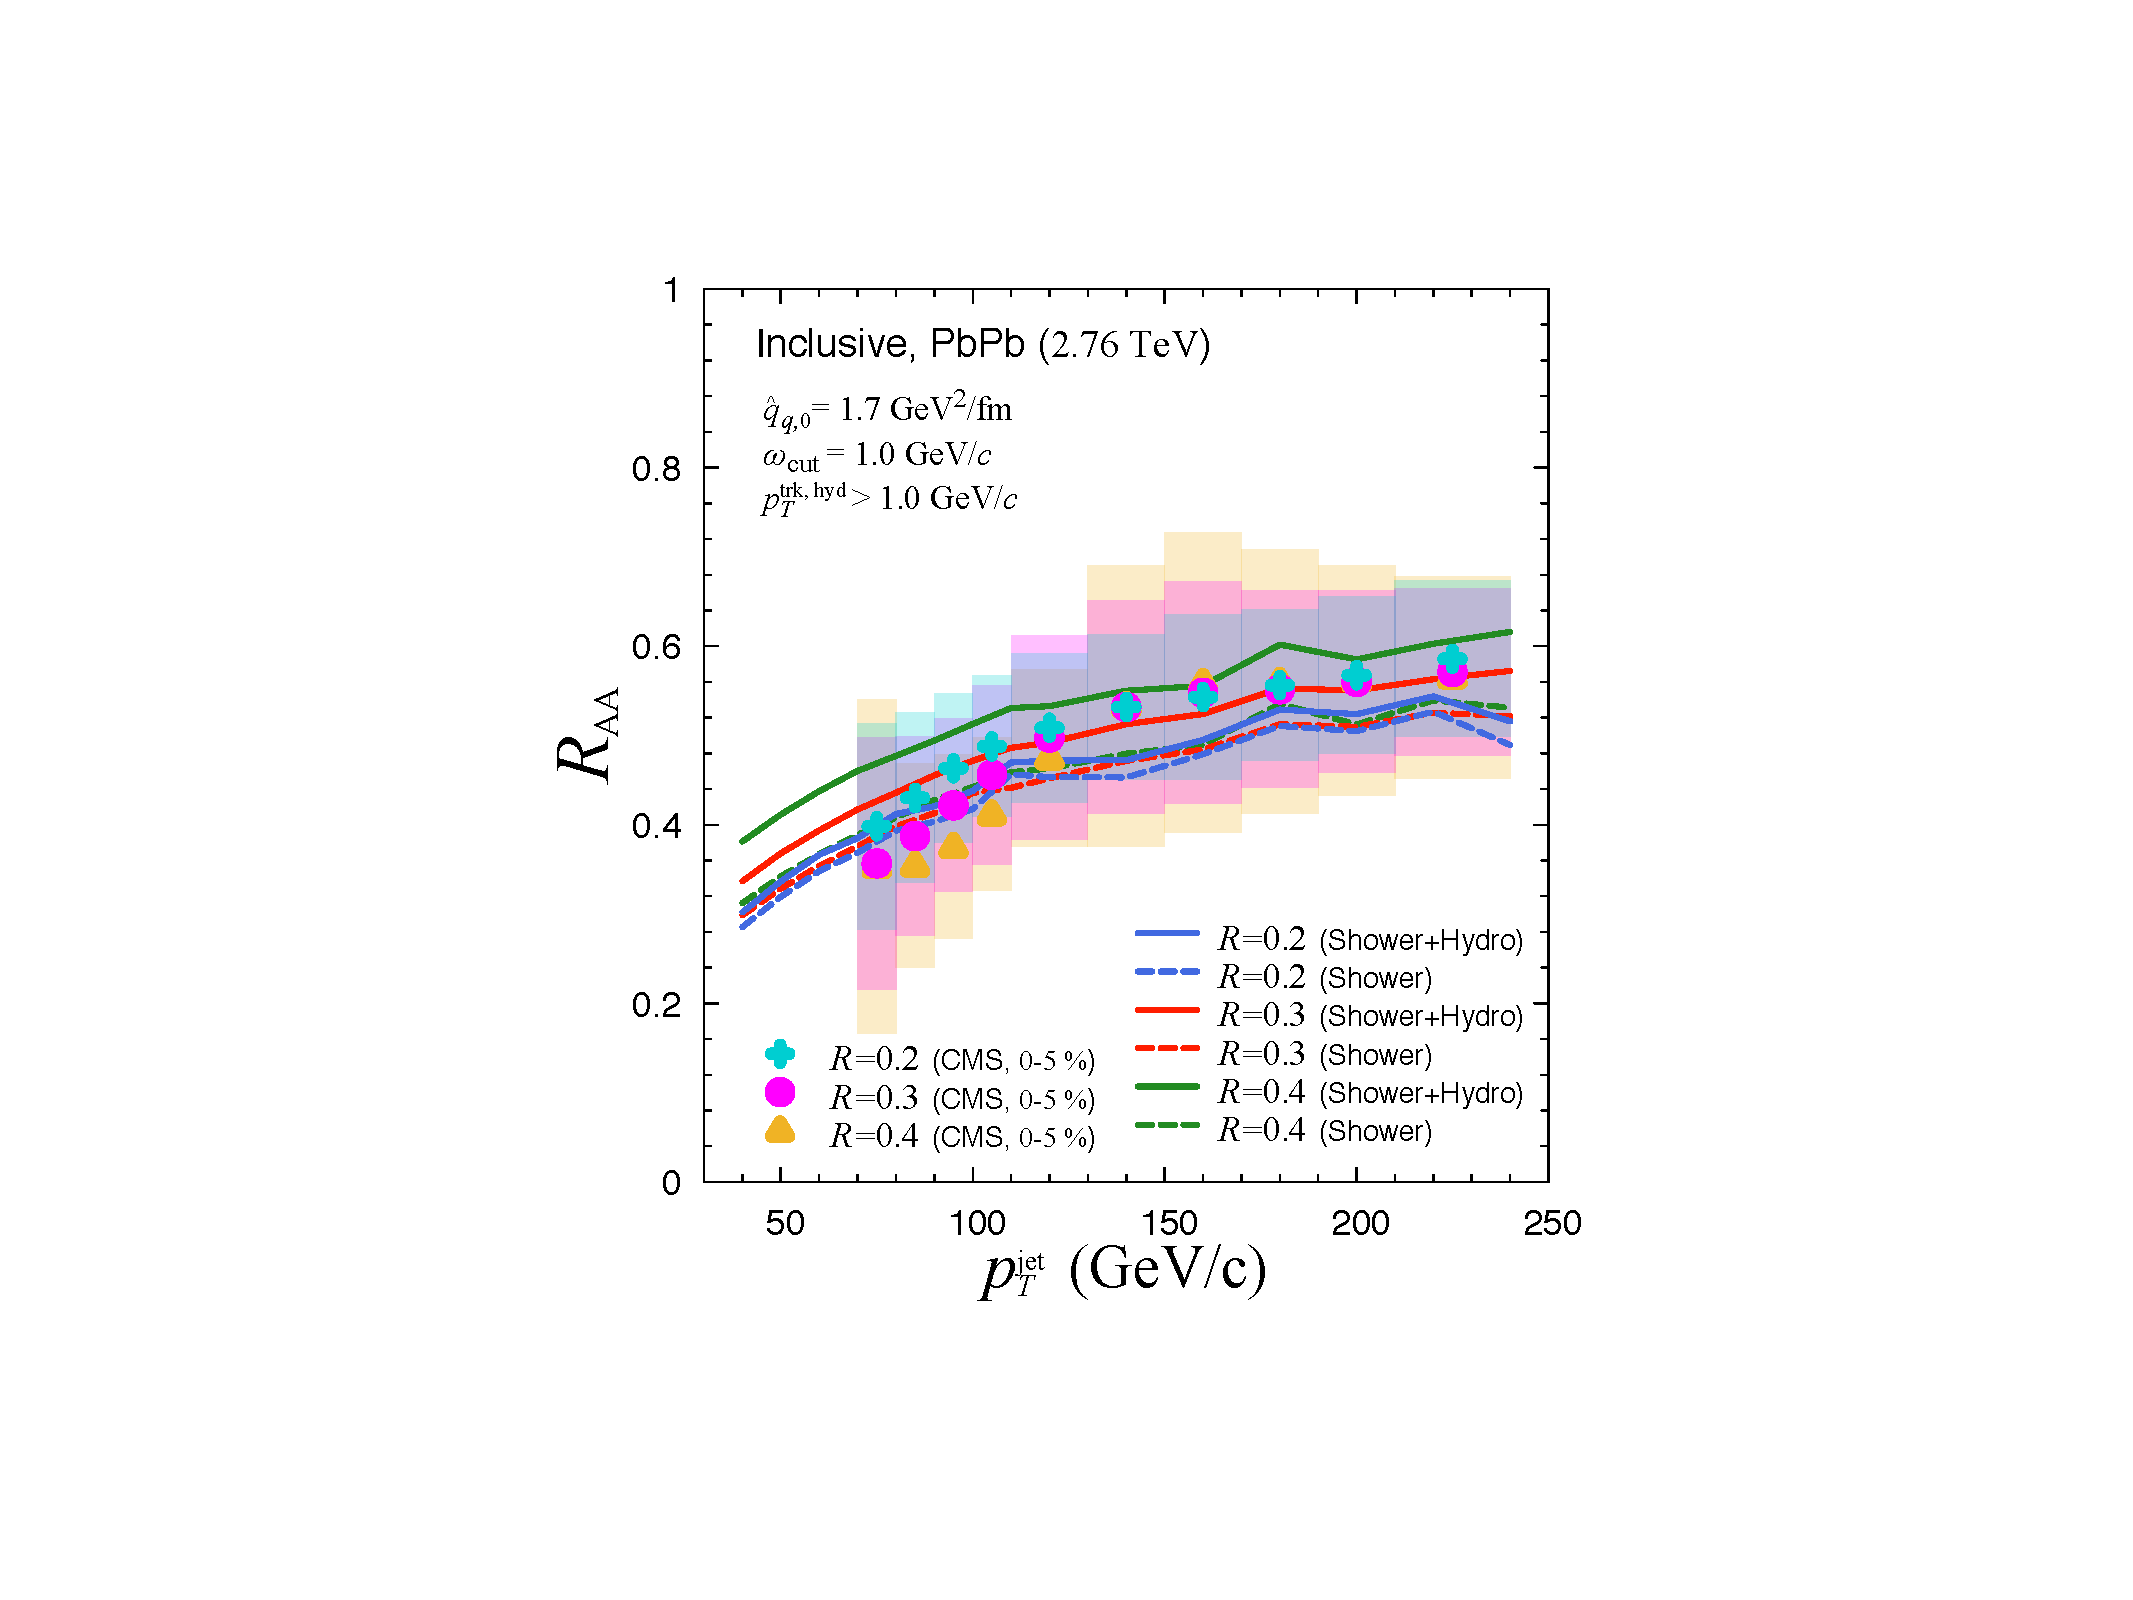
\includegraphics[width=0.45\textwidth]{figures/jetMeasurements/JF_RAA}
\caption{The nuclear modification factor \RAA\ as a function of jet \pt\ as determined by the Jet-Fluid model and compared to the data measured by CMS \cite{Khachatryan:2016jfl}. The different colors represent different sized jets, with the dashed lines showing the modeled \RAA\ without the hydro-contribution. There is good agreement within the large uncertainties in the data. Figure taken from \cite{Tachibana:2017syd}.}
\label{fig:jf_raa}
\end{center}
\end{figure}


The internal structure of the jet, i.e. how energy is spread within it, can be investigated using the jet shape variable, defined as a per-jet quantity as:

\begin{align}
\rho_{\rm jet} = \frac{1}{\Njet} \sum_{\rm jet} \left[ \frac{1}{\ptjet} \frac{\sum_{\rm trk} \pttrk}{\delta r}  \right]
\end{align}
where the sum is over all jets and for all tracks around a jet in an annulus with mean radius $r$ from the jet axis. The modification in the jet structure then can be defined as:

\begin{align}
R_{\rm AA}^\rho = \dfrac{\rho_{\rm AA} (r) }{\rho_{\rm pp} (r) }
\end{align}
A comparison of the jet shape variable $\rho$ and its modification $R_{\rm AA}^\rho$ to data measured by CMS is shown in Figure~\ref{fig:JF_jetShapemodel}. The individual shower and hydro contributions are seen in Figure~\ref{fig:jf_jetshape}. These indicate that the shower contribution to the jet shape variable is falls steeply as a function of distance from the jet axis while the hydro contribution is fairly constant at large distances. This is because the energy loss from the shower is carried away by the jet induced flow to large angles.
The $R_{\rm AA}^\rho$ distribution in Figure~\ref{fig:jf_jetshapemod}, shows that the core is largely unmodified while the outer part of the jet is broadened. The hydro-contribution mainly has an effect at larger distances from the jet axis. This is consistent with the cone-size dependence seen in Figure~\ref{fig:jf_energyLoss}.


\begin{figure}
\begin{subfigure}{.45\textwidth}
  \centering
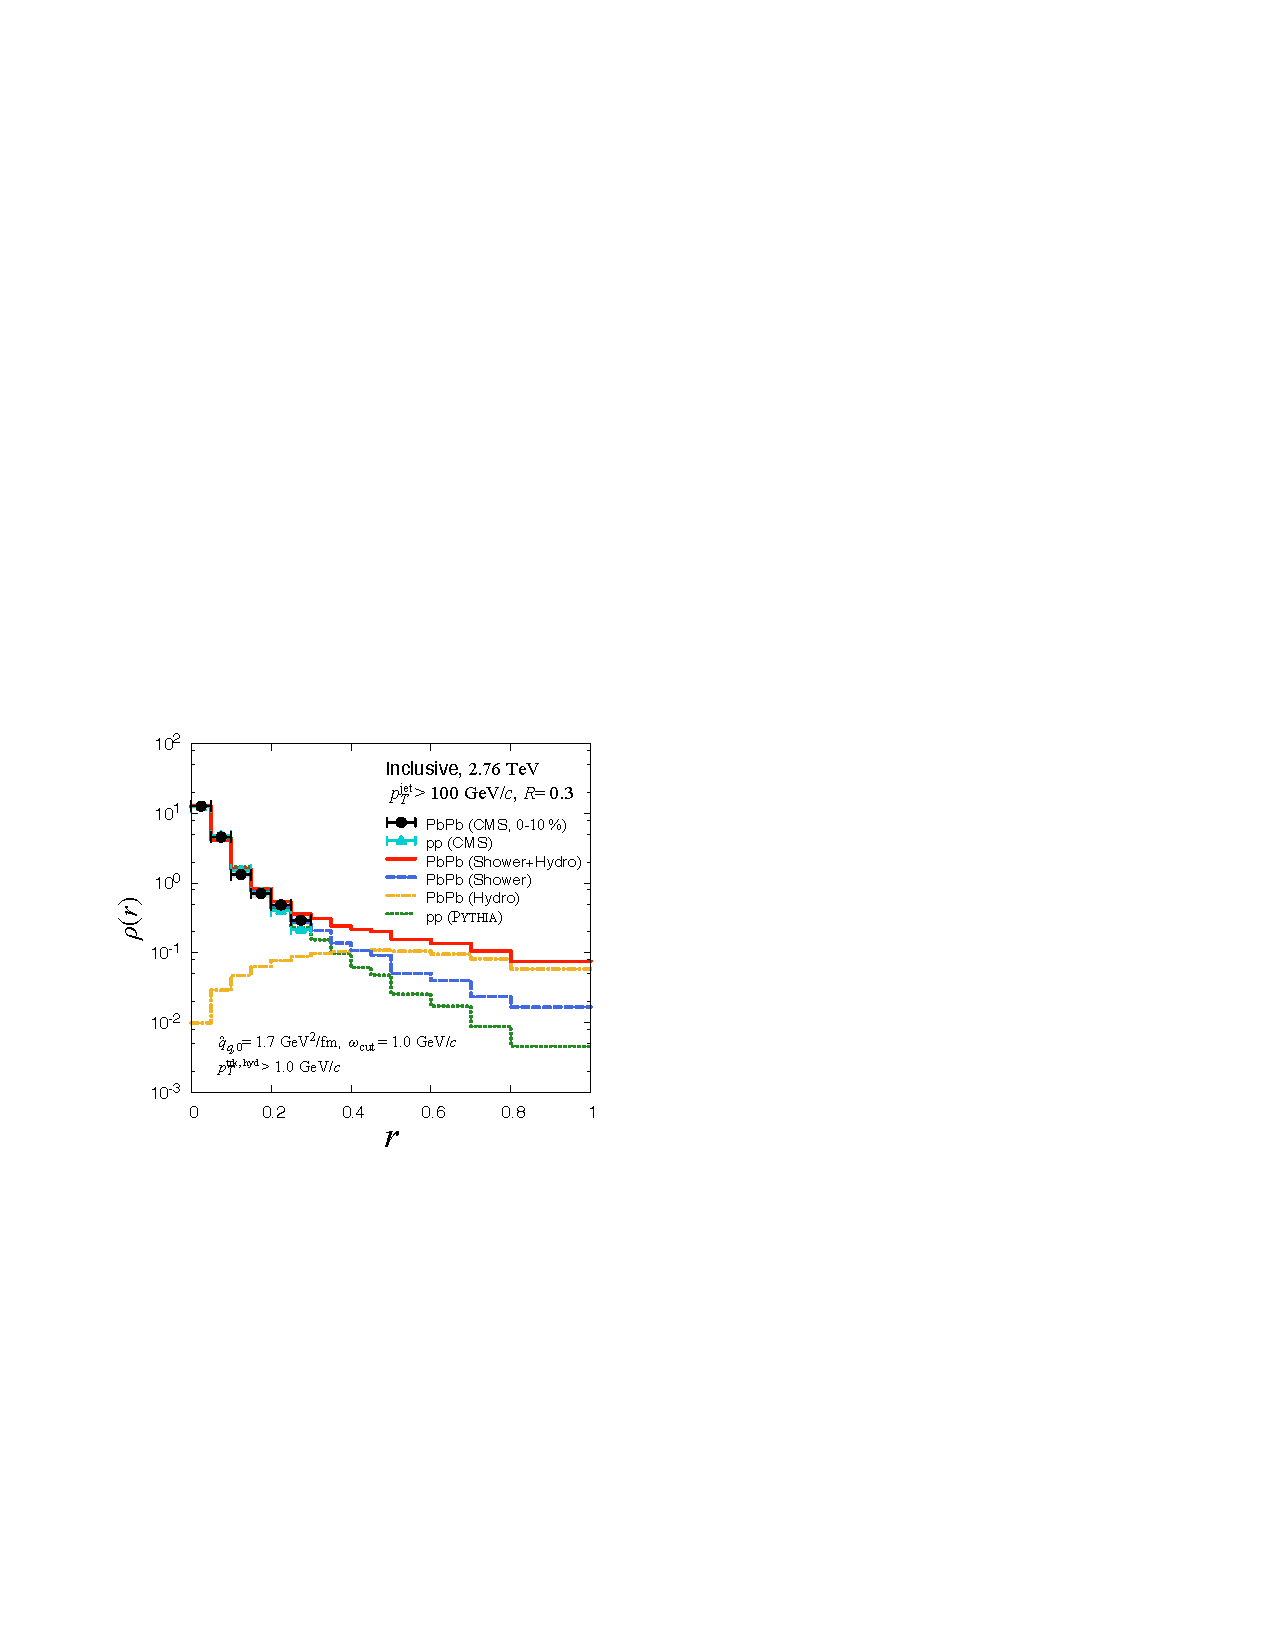
\includegraphics[width=0.95\textwidth]{figures/jetMeasurements/JF_jetShape}
\caption{The jet shape as measured by CMS for \pp\ and central \pbpb\ collisions \cite{Chatrchyan:2013kwa} compared to the Jet Fluid model. The shower (blue) and hydro (orange) contributions to the jet shape are highlighted. Figure taken from \cite{Tachibana:2017syd}.}
\label{fig:jf_jetshape}
\end{subfigure} \qquad
\begin{subfigure}{.45\textwidth}
  \centering
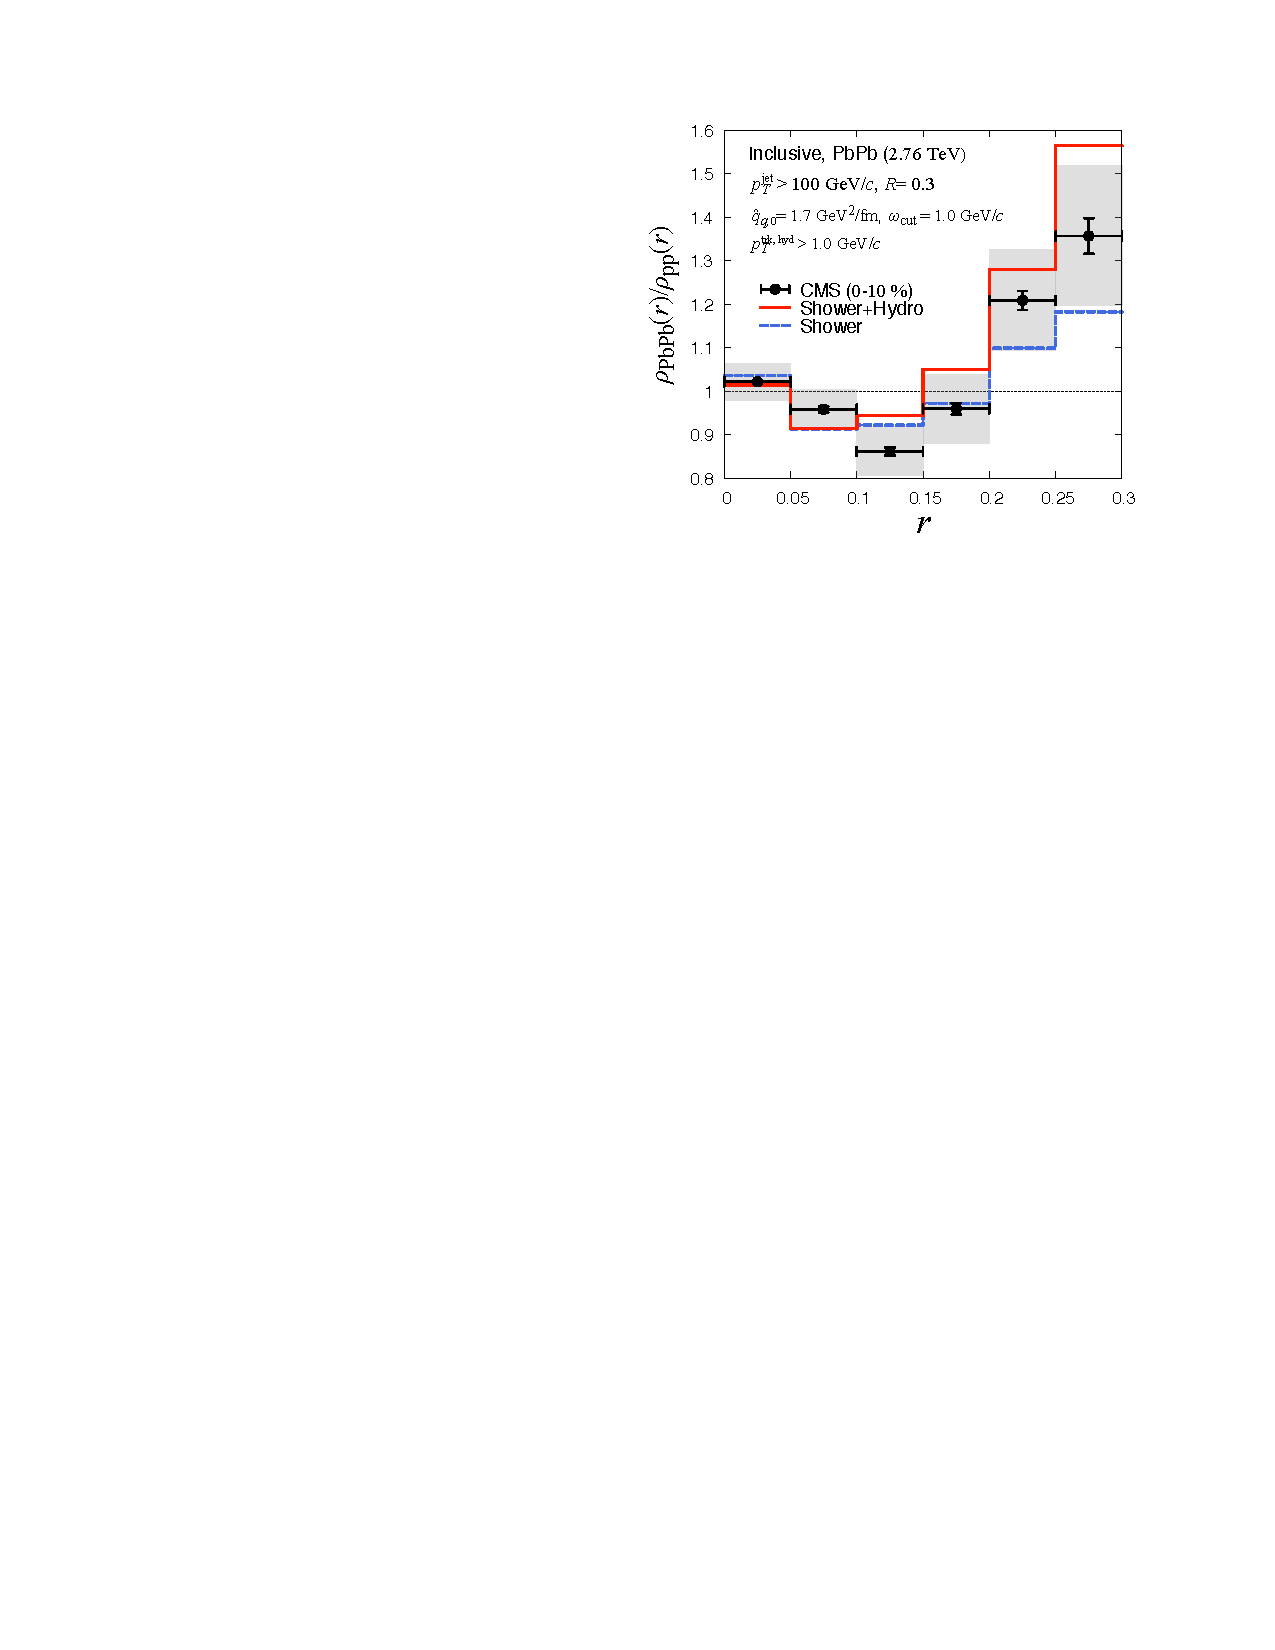
\includegraphics[width=0.95\textwidth]{figures/jetMeasurements/JF_jetShapeModification}
\caption{The modification of the jet shape between \pp\ and \pbpb\ as measured by CMS \cite{Chatrchyan:2013kwa} and compared to the Jet Fluid model. The dashed line shows the modeled modification without the hydro-contribution. Figure taken from \cite{Tachibana:2017syd}.}
\label{fig:jf_jetshapemod}
\end{subfigure}
\caption{Fits to quark fractions and fragmentation functions from \pythia8.  Figure taken from \cite{Spousta:2015fca}}
\label{fig:JF_jetShapemodel}
\end{figure}



%\begin{align}
%\frac{d f_j}{dt} =& \left( \hat{e_j} \frac{\p}{\p \omega_j} + \frac{1}{4} \hat{q_j} \nabla_{\kT}^2\right) f_j  \\
%& + \sum_i \int d\omega_i d\kTsq_i \frac{d\widetilde{\Gamma}_{i\rightarrow j} (\omega_j, \kTsq_j | \omega_i, \kTsq_i)}{d\omega_j d\kTsq dt} f_i \\
%& - \sum_i \int d\omega_i d\kTsq_i \frac{d\widetilde{\Gamma}_{j\rightarrow i} (\omega_i, \kTsq_i | \omega_j, \kTsq_j)}{d\omega_j d\kTsq dt} f_i \\
%\end{align}


%%%%%%%%%%%%%%%%%%%%%%%%%%%%%%%%%%%%%%
\subsection{Hybrid Model}













